% Options for packages loaded elsewhere
\PassOptionsToPackage{unicode}{hyperref}
\PassOptionsToPackage{hyphens}{url}
\PassOptionsToPackage{dvipsnames,svgnames,x11names}{xcolor}
%
\documentclass[
]{article}
\usepackage{amsmath,amssymb}
\usepackage{iftex}
\ifPDFTeX
  \usepackage[T1]{fontenc}
  \usepackage[utf8]{inputenc}
  \usepackage{textcomp} % provide euro and other symbols
\else % if luatex or xetex
  \usepackage{unicode-math} % this also loads fontspec
  \defaultfontfeatures{Scale=MatchLowercase}
  \defaultfontfeatures[\rmfamily]{Ligatures=TeX,Scale=1}
\fi
\usepackage{lmodern}
\ifPDFTeX\else
  % xetex/luatex font selection
\fi
% Use upquote if available, for straight quotes in verbatim environments
\IfFileExists{upquote.sty}{\usepackage{upquote}}{}
\IfFileExists{microtype.sty}{% use microtype if available
  \usepackage[]{microtype}
  \UseMicrotypeSet[protrusion]{basicmath} % disable protrusion for tt fonts
}{}
\makeatletter
\@ifundefined{KOMAClassName}{% if non-KOMA class
  \IfFileExists{parskip.sty}{%
    \usepackage{parskip}
  }{% else
    \setlength{\parindent}{0pt}
    \setlength{\parskip}{6pt plus 2pt minus 1pt}}
}{% if KOMA class
  \KOMAoptions{parskip=half}}
\makeatother
\usepackage{xcolor}
\usepackage[margin=1in]{geometry}
\usepackage{color}
\usepackage{fancyvrb}
\newcommand{\VerbBar}{|}
\newcommand{\VERB}{\Verb[commandchars=\\\{\}]}
\DefineVerbatimEnvironment{Highlighting}{Verbatim}{commandchars=\\\{\}}
% Add ',fontsize=\small' for more characters per line
\usepackage{framed}
\definecolor{shadecolor}{RGB}{248,248,248}
\newenvironment{Shaded}{\begin{snugshade}}{\end{snugshade}}
\newcommand{\AlertTok}[1]{\textcolor[rgb]{0.94,0.16,0.16}{#1}}
\newcommand{\AnnotationTok}[1]{\textcolor[rgb]{0.56,0.35,0.01}{\textbf{\textit{#1}}}}
\newcommand{\AttributeTok}[1]{\textcolor[rgb]{0.13,0.29,0.53}{#1}}
\newcommand{\BaseNTok}[1]{\textcolor[rgb]{0.00,0.00,0.81}{#1}}
\newcommand{\BuiltInTok}[1]{#1}
\newcommand{\CharTok}[1]{\textcolor[rgb]{0.31,0.60,0.02}{#1}}
\newcommand{\CommentTok}[1]{\textcolor[rgb]{0.56,0.35,0.01}{\textit{#1}}}
\newcommand{\CommentVarTok}[1]{\textcolor[rgb]{0.56,0.35,0.01}{\textbf{\textit{#1}}}}
\newcommand{\ConstantTok}[1]{\textcolor[rgb]{0.56,0.35,0.01}{#1}}
\newcommand{\ControlFlowTok}[1]{\textcolor[rgb]{0.13,0.29,0.53}{\textbf{#1}}}
\newcommand{\DataTypeTok}[1]{\textcolor[rgb]{0.13,0.29,0.53}{#1}}
\newcommand{\DecValTok}[1]{\textcolor[rgb]{0.00,0.00,0.81}{#1}}
\newcommand{\DocumentationTok}[1]{\textcolor[rgb]{0.56,0.35,0.01}{\textbf{\textit{#1}}}}
\newcommand{\ErrorTok}[1]{\textcolor[rgb]{0.64,0.00,0.00}{\textbf{#1}}}
\newcommand{\ExtensionTok}[1]{#1}
\newcommand{\FloatTok}[1]{\textcolor[rgb]{0.00,0.00,0.81}{#1}}
\newcommand{\FunctionTok}[1]{\textcolor[rgb]{0.13,0.29,0.53}{\textbf{#1}}}
\newcommand{\ImportTok}[1]{#1}
\newcommand{\InformationTok}[1]{\textcolor[rgb]{0.56,0.35,0.01}{\textbf{\textit{#1}}}}
\newcommand{\KeywordTok}[1]{\textcolor[rgb]{0.13,0.29,0.53}{\textbf{#1}}}
\newcommand{\NormalTok}[1]{#1}
\newcommand{\OperatorTok}[1]{\textcolor[rgb]{0.81,0.36,0.00}{\textbf{#1}}}
\newcommand{\OtherTok}[1]{\textcolor[rgb]{0.56,0.35,0.01}{#1}}
\newcommand{\PreprocessorTok}[1]{\textcolor[rgb]{0.56,0.35,0.01}{\textit{#1}}}
\newcommand{\RegionMarkerTok}[1]{#1}
\newcommand{\SpecialCharTok}[1]{\textcolor[rgb]{0.81,0.36,0.00}{\textbf{#1}}}
\newcommand{\SpecialStringTok}[1]{\textcolor[rgb]{0.31,0.60,0.02}{#1}}
\newcommand{\StringTok}[1]{\textcolor[rgb]{0.31,0.60,0.02}{#1}}
\newcommand{\VariableTok}[1]{\textcolor[rgb]{0.00,0.00,0.00}{#1}}
\newcommand{\VerbatimStringTok}[1]{\textcolor[rgb]{0.31,0.60,0.02}{#1}}
\newcommand{\WarningTok}[1]{\textcolor[rgb]{0.56,0.35,0.01}{\textbf{\textit{#1}}}}
\usepackage{graphicx}
\makeatletter
\def\maxwidth{\ifdim\Gin@nat@width>\linewidth\linewidth\else\Gin@nat@width\fi}
\def\maxheight{\ifdim\Gin@nat@height>\textheight\textheight\else\Gin@nat@height\fi}
\makeatother
% Scale images if necessary, so that they will not overflow the page
% margins by default, and it is still possible to overwrite the defaults
% using explicit options in \includegraphics[width, height, ...]{}
\setkeys{Gin}{width=\maxwidth,height=\maxheight,keepaspectratio}
% Set default figure placement to htbp
\makeatletter
\def\fps@figure{htbp}
\makeatother
\setlength{\emergencystretch}{3em} % prevent overfull lines
\providecommand{\tightlist}{%
  \setlength{\itemsep}{0pt}\setlength{\parskip}{0pt}}
\setcounter{secnumdepth}{-\maxdimen} % remove section numbering
\ifLuaTeX
  \usepackage{selnolig}  % disable illegal ligatures
\fi
\usepackage{bookmark}
\IfFileExists{xurl.sty}{\usepackage{xurl}}{} % add URL line breaks if available
\urlstyle{same}
\hypersetup{
  pdftitle={Projet IF36},
  pdfauthor={Baptiste Toussaint},
  colorlinks=true,
  linkcolor={Maroon},
  filecolor={Maroon},
  citecolor={Blue},
  urlcolor={blue},
  pdfcreator={LaTeX via pandoc}}

\title{Projet IF36}
\author{Baptiste Toussaint}
\date{2024-06-11}

\begin{document}
\maketitle

\section{Analyse : GitHub Public Repository
Metadata}\label{analyse-github-public-repository-metadata}

\begin{quote}
Projet de \emph{Data visualization} de l'unité d'enseignement IF36 de
l'\href{https://www.utt.fr/}{Université de Technologie de Troyes (UTT)}.
\end{quote}

Nom du groupe : \textbf{\emph{La cité de la}} f \textbf{\emph{eur}}.

Membres : \href{https://github.com/I3at57}{Baptiste Toussaint},
\href{https://github.com/yvlann}{XU Shilun},
\href{https://github.com/louisduhalberruer}{Louis Duhal Berruer}

Langue : Français

\begin{center}\rule{0.5\linewidth}{0.5pt}\end{center}

\section{1. Introduction}\label{introduction}

\subsection{1.1 Description des
données.}\label{description-des-donnuxe9es.}

\subsubsection{1.1.1 Présentation de
GitHub}\label{pruxe9sentation-de-github}

\begin{figure}
\centering

\includegraphics[width=0.2\textwidth,height=0.2\textheight]{./src/img/GitHub_Logo.png}
\caption{Logo de la mascotte de GitHub}
\end{figure}

\begin{figure}
\centering

\includegraphics[width=0.2\textwidth,height=0.2\textheight]{./src/img/github-mark.png}
\caption{Logo de GitHub}
\end{figure}

\begin{quote}
Logo de GitHub et de sa mascotte : Octocat
\end{quote}

\href{https://github.com/}{\emph{GitHub}} est un service web à
destination des développeurs permettant d'héberger, partager, et
versionner du code. Initialement conçu comme outil complémentaire à
\emph{Git} pour le contrôle de version, \emph{GitHub} est aujourd'hui
une véritable plateforme de développement utilisée par plus de 100
millions d'utilisateurs à travers le monde.

\emph{GitHub} voit le jour en 2008 et s'impose rapidement comme l'outil
d'hébergement en ligne privilégié des développeurs, en particulier dans
la communauté des projet open source et libres de droit.

La plateforme propose une offre gratuite performante permettant à
n'importe quelle équipe de créer et faire vivre leurs projets en ligne.
Elle propose aussi des offres payantes pour les entreprises de plus
grande taille.

Ainsi, il est possible de retrouver sur GitHub le code de grandes
compagnies comme \href{https://github.com/google}{\emph{Google}} ou
\href{https://github.com/microsoft/}{\emph{Microsoft}}.

Sur \emph{GitHub}, les utilisateurs créent des \textbf{dépôts} (en
anglais \emph{repositories} ou \emph{repo} pour la version courte) qui
accueillent l'ensemble des fichiers d'un programme, un logiciel, etc.

Le 8 novembre dernier, l'entreprise \emph{GitHub} déclarait alors près
de 420 millions de projets présents sur la plateforme, dont 284 millions
publics.

\subsubsection{1.1.2 Les métadonnées de l'API
GitHub}\label{les-muxe9tadonnuxe9es-de-lapi-github}

GitHub met à disposition une
\href{https://docs.github.com/en/rest/about-the-rest-api/about-the-rest-api?apiVersion=2022-11-28}{API}
permettant aux utilisateurs d'automatiser une série de tâches en lien
avec le service. Cette API peut notamment être utilisée pour récupérer
des informations relatives à la télémétrie des dépôts : nom du dépôt,
nombre de contributeur, dates des contributions, etc.

L'utilisateur \href{https://pelmers.com/blog/}{Peter Elmers} a développé
un \href{https://github.com/pelmers/github-repository-metadata}{script}
qui utilise cette API pour extraire les informations (\emph{scraping})
d'environ trois millions de \emph{repo} publics.

Il est important de noter que le fichier JSON de Peter Elmers ne
contient que des repos publiques (visibles de tous) possédants au
minimum 5 étoiles (l'équivalent des \emph{like} sur la plateforme
github).

Le résultat de ce script est un fichier JSON hébergé sur la plateforme
\href{https://www.kaggle.com/datasets/pelmers/github-repository-metadata-with-5-stars/data}{Kaggle}.

La dernière mise à jour du jeu de donnée date du 25 février 2024. Les
données sont donc actuelles et toujours pertinentes à analyser.

De plus, le jeu de données est partagé sous license : ``Attribution 4.0
International (CC BY 4.0)''.

Pour faciliter la manipulation des données, nous avons décidé de ne
conserver que les 200000 premières entrées de ce fichier JSON pour le
moment. Cela correspond aux 200000 repos possédant le plus
\emph{d'étoiles} sur la plateforme (les repos les plus \emph{likés} si
l'on peut se permettre cette analogie).

Nous pourrons sans problème ajouter des données durant notre analyse si
nous en ressentons le besoin.

Nous n'excluons pas non plus de recourir à l'API de GitHub pour
augmenter les données pour améliorer l'analyse.

Afin de résoudre le problème des fichiers json trop lourd, nous avons
décidé d'exécuter le code python suivant dans un notebook sur Kaggle
pour exporter les données par sections en format de CSV:

\begin{verbatim}
import pandas as pd

# read json file
json_file_path = '/kaggle/input/github-repository-metadata-with-5-stars/repo_metadata.json'
df = pd.read_json(json_file_path)

# every chunk row
chunk_size = 10000

# calculate rows
total_rows = df.shape[0]

# calculate the number of files
num_files = (total_rows + chunk_size - 1) // chunk_size

# split and output files
for i in range(num_files):
    start_idx = i * chunk_size
    end_idx = min((i + 1) * chunk_size, total_rows)
    
    # get current data
    chunk_df = df.iloc[start_idx:end_idx]
    
    # generate file path
    output_file_path = f'/kaggle/working/data_{i + 1}.csv'
    
    # output data to csv
    chunk_df.to_csv(output_file_path, index=False)

    print(f'File {i + 1} written to {output_file_path}')
\end{verbatim}

Nous avons donc dix fichiers nommés \texttt{data\_X.csv} numérotés de 1
à 10. Les dix premiers fichiers sont rangés dans le dossier :
\texttt{githubStar1-10}, les dix suivants sont rangés dans le dossier :
\texttt{githubStar11-20}.

Nous avons ensuite regroupé les données de ces vingts fichiers dans un
unique fichier nommé \texttt{data\_1\_200000.csv} pour en faciliter la
manipulation.

Ces fichiers se trouvent dans le dossier \texttt{./data/} de ce dépôt.

\subsubsection{1.1.3 Présentation des
données}\label{pruxe9sentation-des-donnuxe9es}

Le jeu de données contient donc environ trois millions de dépôts
publics, tous ayant plus de cinq étoiles (nous reviendrons plus loin sur
la signification de ces étoiles).

Chaque objet du fichier JSON représente un dépôt décrit par les
variables suivantes (description mise en ligne par Peter Elmer
\href{https://github.com/pelmers/github-repository-metadata}{ici}).

\begin{itemize}
\item
  \texttt{owner}, propriétaire ou créateur du dépôt, identifié par son
  nom d'utilisateur sur la plateforme GitHub. {[}type :
  \texttt{string}{]} ;
\item
  \texttt{name}, nom du dépôt. {[}type : \texttt{string}{]} ;
\item
  \texttt{stars}, nombre d'étoiles, de \emph{like} du dépôt. {[}type :
  \texttt{int}{]} ;
\item
  \texttt{forks}, nombre de \emph{fork} du projet. {[}type :
  \texttt{int}{]} ;
\item
  \texttt{watchers}, nombre d'utilisateurs surveillant le projet.
  {[}type : \texttt{int}{]} ;
\item
  \texttt{isFork}, précise si le dépôt est un \emph{fork} d'un autre
  dépôt. {[}type:\texttt{bool}{]} ;
\item
  \texttt{isArchived}, précise si le dépôt est archivé ou non. {[}type
  :\texttt{bool}{]} ;
\item
  \texttt{languages}, une structure de type \texttt{list} regroupant les
  langages de programmation utilisés dans le projet. Chaque élément de
  la liste est composé du nom du langage et de la taille en octet,
  consacré à ce langage dans le dépôt. {[}type : \texttt{list}{]} ;
\item
  \texttt{languageCount}, nombre de langage utilisés. {[}type :
  \texttt{int}{]} ;
\item
  \texttt{topics}, une structure de type \texttt{list} regroupant les
  \emph{topics} associés au dépôt. Pour chaque \emph{topic} on retrouve
  le nom et le nombre d'étoiles associées pour ce \emph{topic} sur
  l'ensemble de la plateforme. Les \emph{topic} permettent aux créateurs
  des dépôts d'identifier les objectifs ou catégories de leurs projets.
  Cela ressemble au système des \emph{hashtag} popularisé par
  \emph{Twitter}. {[}type : \texttt{list}{]} ;
\item
  \texttt{topicCount}, nombre de \emph{topic} associés au dépôt. {[}type
  : \texttt{int}{]} ;
\item
  \texttt{diskUsageKb}, taille du dépôt en kB. {[}type : \texttt{int}{]}
  ;
\item
  \texttt{pullRequests}, nombre de \emph{pull request}. {[}type :
  \texttt{int}{]} ;
\item
  \texttt{issues}, nombre d'\emph{issues}. {[}type : \texttt{int}{]} ;
\item
  \texttt{description}, description du \emph{repo}. {[}type :
  \texttt{string}{]} ;
\item
  \texttt{primaryLanguage}, nom du langage de programmation
  principalement dans le projet. {[}type : \texttt{string}{]} ;
\item
  \texttt{createdAt}, date de création du dépôt. La date est au format :
  ``AAAA-MM-JJTHH:MM:SSZ'', par exemple : ``2015-03-14T22:35:11Z''.
  Attention cependant, il faudra préciser quel fuseau horaire est
  utilisé par l'API pour ne pas fausser n'analyse. {[}type :
  \texttt{string}{]} ;
\item
  \texttt{pushedAt}, dernière date de \emph{push} du projet, soit la
  dernière date de mise à jour du dépôt par un contributeur. Le format
  est identique à l'attribut \texttt{createdAt}. {[}type :
  \texttt{string}{]} ;
\item
  \texttt{defaultBranchCommitCount}, nombre de \emph{commit} sur la
  \emph{branche principale}. Nous rentrerons dans l'explication complète
  du système de \emph{commit} dans l'analyse des données. À ce stade on
  peut approximer le nombre de \emph{commit} comme le nombre de version
  du projet. {[}type : \texttt{int}{]} ;
\item
  \texttt{license}, licence utilisée par le projet. Permet de connaître
  les droits donnés aux utilisateurs.
\item
  \texttt{assignableUserCount}, nombre d'utilisateurs ayant des droits
  d'accès sur le projet. {[}type : \texttt{int}{]} ;
\item
  \texttt{codeOfConduct}, si le projet possède un code de bonne conduite
  pour ses utilisateurs (règles de communauté), mentionne son nom.
  {[}type : \texttt{string}{]} ;
\item
  \texttt{forkingAllowed}, indique s'il est possible de \emph{fork} le
  projet : s'il est possible d'en faire une copie. Indique vrai ou faux
  : \texttt{TRUE} ou \texttt{FALSE}. {[}type : \texttt{bool}{]} ;
\item
  \texttt{nameWithOwner}, concaténation du nom du dépôt avec le nom du
  créateur. {[}type : \texttt{string}{]} ;
\item
  \texttt{parent}, indique le nom du dépôt parent si ce dépôt est un
  \emph{fork}. {[}type : \texttt{string}{]}.
\end{itemize}

\subsubsection{1.1.4 Pourquoi étudier ces données
?}\label{pourquoi-uxe9tudier-ces-donnuxe9es}

Nous sommes trois étudiants de l'UTT avec un parcours tourné vers
l'informatique, les nouvelles technologies et la programmation.

GitHub est une plateforme que nous utilisons personnellement (en plus de
l'utiliser pour ce projet) de manières différentes : les langages de
programmation utilisées dans la branche ISI de l'UTT sont différents des
langages utilisés en branche GI par exemple.

L'avantage de ce jeu de données est de permettre de présenter les
langages de programmations utilisés dans les projets les plus
``populaires'' de la plateforme et pourquoi pas de comparer nos
résultats avec nos langages préférés.

Ce travail d'analyse des tendance est déjà fait par GitHub chaque années
à travers ces articles \href{https://octoverse.github.com/}{Octoverse
report}.

\begin{center}\rule{0.5\linewidth}{0.5pt}\end{center}

\subsection{1.2 Plan d'analyse}\label{plan-danalyse}

\subsubsection{1.2.1 Objectifs de
l'analyses}\label{objectifs-de-lanalyses}

Nous possédons donc les entrées relatives aux 200000 dépôts les plus
\emph{likés} de GitHub (ceux ayant obtenu les plus d'étoiles :
\emph{stars} ).

Dans un premier temps, nous nous demanderons comment se répartissent les
\emph{stars} de notre population.

On peut s'attendre à ce qu'une petite partie de projet possèdent un
nombre important d'étoile, et ce nombre décroit rapidement, comme une
exponentielle décroissante.

Si l'on s'en tient au principe de
\href{https://fr.wikipedia.org/wiki/Principe_de_Pareto}{Pareto}
(principe du 80/20), on peut penser que 20\% des dépôts sur GitHub
concentrent 80\% du nombre total d'étoiles attribués par les
utilisateurs. Cette hypothèse n'est pas déraisonnable, puisque que ce
principe est applicable dans beaucoup de domaine.

Bien que le principe de
\href{https://fr.wikipedia.org/wiki/Principe_de_Pareto}{Pareto} ne soit
pas une règle parfaite, c'est en général une première approche naïve
utile pour appréhender des phénomènes.

Si l'on considère GitHub comme un réseaux social, et que l'on considère
que les \emph{stars} d'un projet mesurent sa ``popularité'', nous
chercherons dans la suite de l'étude à trouver ce qui peut expliquer la
popularité d'un projet sur \emph{GitHub}.

Nous allons donc lier la caractéristique du nombre d'étoile avec les
autres paramètres de notre jeu de données.

\subsubsection{1.2.2 Mesure de la
popularité}\label{mesure-de-la-popularituxe9}

Nous disposons de la date de création des dépôts (notre jeu de données
contient des dépôts créés entre 2009 et 2023), nous pourrons chercher
s'il existe une corrélation entre la date de création et la popularité
du projet. En effet on peut penser que les dépôts les plus anciens sont
les dépôts les plus appréciées.

Avec le nombre de \emph{fork} (ou clonage en français) par dépôt nous
pourront essayer de voir si les projets les plus aimés sont aussi les
projets les plus repris par les utilisateurs.

Quand un utilisateur \emph{fork} un dépôt, il en crée une copie
personnelle sur laquelle il est libre d'ajouter les modifications qu'il
souhaite.

Le nombre de clonage peut être un indicateur supplémentaire de
popularité et on peut chercher à savoir si cet indicateur est corrélé au
nombre d'étoile d'un projet.

Le paramètre \emph{watchers} est une donnée supplémentaire d'analyse de
``popularité''. Quand un utilisateur \emph{watchs} (que l'on peut
traduire par surveiller ou suivre, en français) un projet, il est averti
quand ce dernier subit une modification.

Là encore, on pourra chercher à vérifier l'existence d'une corrélation
entre le nombre d'étoile, le nombre de clone, et le nombre de suivi des
dépôts.

\subsubsection{1.2.3 Mesure des
contributions}\label{mesure-des-contributions}

GitHub est énormément utilisé par les projets collaboratifs pour
permettre aux développeurs du monde entier de contribuer à des projets.

Selon leurs politiques de gouvernance, les propriétaires de dépôts
peuvent permettre à certains utilisateurs autorisés ou à n'importe quel
contributeur de proposer des modifications (les \emph{pullRequests}) ou
signaler des bugs (les \emph{issues}).

On dispose donc de ces deux indicateurs qui permettent de quantifier
l'interactivité d'un projet : plus ces deux valeurs sont grandes, plus
on peut considérer le projet comme actif.

Nous ne disposons cependant pas du nombre de contributeurs par dépôt.
L'attribut : \texttt{assignableUserCount} semble uniquement représenter
le nombre de contributeurs ayant des droits d'accès spécifiques.

Nous pourrons par exemple utiliser l'API pour augmenter notre jeu de
données et trouver pour chaque dépôt le nombre de contributeur réel.

\subsubsection{1.2.4 Étude des langages de programmation
utilisés}\label{uxe9tude-des-langages-de-programmation-utilisuxe9s}

Nous pourrons ensuite analyser les types de langage utilisés.

Nous chercherons à faire une cartographie des langages les plus utilisés
et nous pourrons peut-être lier cette analyse avec la popularité des
dépôts : existe-t-il des langages plus populaires que les autres ?

On peut supposer par exemple que les dépôts très populaires ne
contiennent pas de \emph{Pascal} ou d'\emph{Ada}\ldots{}

\subsubsection{\texorpdfstring{1.2.5 Prise en compte des
\emph{topics}}{1.2.5 Prise en compte des topics}}\label{prise-en-compte-des-topics}

Toute notre analyse jusqu'ici repose sur une hypothèse : les dépôts
GitHub ne contiennent que des projets de programmation ou de code.

Cette hypothèse est fausse ! En effet, avec sa démocratisation, GitHub a
connu une diversification des usages.

Aujourd'hui en tant que véritable réseau social pour développeurs et
geek en tous genres, certains utilise la plateforme pour créer des
portfolios en ligne, des pages vitrines pour un site ou un service, etc.

Par exemple, le dépôt :
\href{https://github.com/papers-we-love/papers-we-love}{papers-we-love}
est une immense compilation de papiers scientifiques relatifs à
l'informatique.

Il est donc très difficile de comparer ce genre de dépôt avec des
projets informatiques.

L'attribut \texttt{topics} du dataset peut nous aider à classifier les
dépôts selon leurs objectifs et catégories identifiées : projets,
vitrines, listes, cours, etc.

Il sera possible d'effectuer une analyse croisée entre les langages et
les \emph{topics} pour observer quels \emph{topics} sont associés à
quels langages.

Le créateur du dataset, Peter Elmer, propose sur la page kaggle une
représentation de type \emph{word clouds} montrant les \emph{topics} les
plus représentés par langage de programmation.

Nous pourrons essayer de reproduire ce résultat, d'autant qu'il n'a pas
partagé le code correspondant.

\subsection{1.3 Préparation des
données}\label{pruxe9paration-des-donnuxe9es}

\subsubsection{1.3.1 Charger le jeu de
données}\label{charger-le-jeu-de-donnuxe9es}

\begin{Shaded}
\begin{Highlighting}[]
\CommentTok{\# Chagre les librairies utiles}
\FunctionTok{library}\NormalTok{(tidyverse)}
\end{Highlighting}
\end{Shaded}

\begin{verbatim}
## Warning: package 'tidyverse' was built under R version 4.3.3
\end{verbatim}

\begin{verbatim}
## -- Attaching core tidyverse packages ------------------------ tidyverse 2.0.0 --
## v dplyr     1.1.4     v readr     2.1.5
## v forcats   1.0.0     v stringr   1.5.1
## v ggplot2   3.5.0     v tibble    3.2.1
## v lubridate 1.9.3     v tidyr     1.3.1
## v purrr     1.0.2     
## -- Conflicts ------------------------------------------ tidyverse_conflicts() --
## x dplyr::filter() masks stats::filter()
## x dplyr::lag()    masks stats::lag()
## i Use the conflicted package (<http://conflicted.r-lib.org/>) to force all conflicts to become errors
\end{verbatim}

\begin{Shaded}
\begin{Highlighting}[]
\FunctionTok{library}\NormalTok{(ggrepel)}
\end{Highlighting}
\end{Shaded}

\begin{verbatim}
## Warning: package 'ggrepel' was built under R version 4.3.3
\end{verbatim}

\begin{Shaded}
\begin{Highlighting}[]
\CommentTok{\# thème pour les graphiques}
\NormalTok{custom\_theme }\OtherTok{\textless{}{-}} \FunctionTok{theme}\NormalTok{(}
        \AttributeTok{panel.background =} \FunctionTok{element\_rect}\NormalTok{(}\AttributeTok{fill =} \StringTok{"\#D9E8F1"}\NormalTok{,}
                                        \AttributeTok{colour =} \StringTok{"\#6D9EC1"}\NormalTok{,}
                                        \AttributeTok{size =} \DecValTok{1}\NormalTok{, }\AttributeTok{linetype =} \StringTok{"solid"}\NormalTok{)}
\NormalTok{)}
\end{Highlighting}
\end{Shaded}

\begin{verbatim}
## Warning: The `size` argument of `element_rect()` is deprecated as of ggplot2 3.4.0.
## i Please use the `linewidth` argument instead.
## This warning is displayed once every 8 hours.
## Call `lifecycle::last_lifecycle_warnings()` to see where this warning was
## generated.
\end{verbatim}

Dans le dossier
\texttt{.\textbackslash{}data\textbackslash{}githubStar1-10\textbackslash{}}
on dispose de 10 fichiers \texttt{.csv} qui possèdent 10000 éléments
chacun soit 100000 éléments.

Je propose un petit script pour fusionner ces fichiers en un seul
fichier commun pour simplifier la manipulation :

Pour vérifier :

\begin{Shaded}
\begin{Highlighting}[]
\CommentTok{\# Si besoin de charger le dataset}
\NormalTok{df }\OtherTok{\textless{}{-}} \FunctionTok{read\_csv}\NormalTok{(}\StringTok{"../../data/data\_1\_200000.csv"}\NormalTok{)}
\end{Highlighting}
\end{Shaded}

\begin{verbatim}
## Rows: 200000 Columns: 25
## -- Column specification --------------------------------------------------------
## Delimiter: ","
## chr   (9): owner, name, languages, topics, description, primaryLanguage, lic...
## dbl  (10): stars, forks, watchers, languageCount, topicCount, diskUsageKb, p...
## lgl   (4): isFork, isArchived, forkingAllowed, parent
## dttm  (2): createdAt, pushedAt
## 
## i Use `spec()` to retrieve the full column specification for this data.
## i Specify the column types or set `show_col_types = FALSE` to quiet this message.
\end{verbatim}

\subsubsection{1.3.2 Triater les doublons}\label{triater-les-doublons}

Pour commencer nous devons nettoyer le dataset en identifiant les
possibles doublons.

\begin{Shaded}
\begin{Highlighting}[]
\FunctionTok{dim}\NormalTok{(df)[}\DecValTok{1}\NormalTok{] }\SpecialCharTok{{-}} \FunctionTok{dim}\NormalTok{(}\FunctionTok{unique}\NormalTok{(df))[}\DecValTok{1}\NormalTok{] }\CommentTok{\# Nombre de doublons}
\end{Highlighting}
\end{Shaded}

\begin{verbatim}
## [1] 5804
\end{verbatim}

Nous avons à priori 5804 doublons.

\begin{Shaded}
\begin{Highlighting}[]
\NormalTok{df\_duplicates }\OtherTok{\textless{}{-}}\NormalTok{ df[}\FunctionTok{duplicated}\NormalTok{(df),] }\CommentTok{\# stock les doublons dans un objet}
\FunctionTok{head}\NormalTok{(df\_duplicates) }\CommentTok{\# Montre les premières lignes des doublons}
\end{Highlighting}
\end{Shaded}

\begin{verbatim}
## # A tibble: 6 x 25
##   owner     name  stars forks watchers isFork isArchived languages languageCount
##   <chr>     <chr> <dbl> <dbl>    <dbl> <lgl>  <lgl>      <chr>             <dbl>
## 1 FFmpeg    FFmp~ 37824 11218     1379 FALSE  FALSE      [{'name'~            15
## 2 labstack  echo  26331  2180      523 FALSE  FALSE      [{'name'~             3
## 3 alibaba   canal 26312  7356     1198 FALSE  FALSE      [{'name'~            11
## 4 floating~ floa~ 26311  1523      254 FALSE  FALSE      [{'name'~             6
## 5 portainer port~ 26277  2223      471 FALSE  FALSE      [{'name'~            11
## 6 lukasz-m~ awes~ 26258  2638      988 FALSE  FALSE      []                    0
## # i 16 more variables: topics <chr>, topicCount <dbl>, diskUsageKb <dbl>,
## #   pullRequests <dbl>, issues <dbl>, description <chr>, primaryLanguage <chr>,
## #   createdAt <dttm>, pushedAt <dttm>, defaultBranchCommitCount <dbl>,
## #   license <chr>, assignableUserCount <dbl>, codeOfConduct <chr>,
## #   forkingAllowed <lgl>, nameWithOwner <chr>, parent <lgl>
\end{verbatim}

\begin{Shaded}
\begin{Highlighting}[]
\NormalTok{df }\OtherTok{\textless{}{-}} \FunctionTok{unique}\NormalTok{(df) }\CommentTok{\# retire les doublons au dataset df}
\NormalTok{n }\OtherTok{\textless{}{-}} \FunctionTok{dim}\NormalTok{(df)[}\DecValTok{1}\NormalTok{]}
\NormalTok{m }\OtherTok{\textless{}{-}} \FunctionTok{dim}\NormalTok{(df)[}\DecValTok{2}\NormalTok{]}
\end{Highlighting}
\end{Shaded}

\section{2. Première étude : mesurer la popularité des
dépôts}\label{premiuxe8re-uxe9tude-mesurer-la-popularituxe9-des-duxe9puxf4ts}

\subsection{2.1 Notre interprétation du nombre d'étoile d'un dépôt sur
GitHub}\label{notre-interpruxe9tation-du-nombre-duxe9toile-dun-duxe9puxf4t-sur-github}

Le fichier \texttt{data\_1\_200000.csv} contenu dans l'objet \texttt{df}
contient les 200000 dépôts possédant le plus d'étoiles
(\textbf{\emph{stars}}) sur GitHub au 25 février 2024.

Sur GitHub, les étoiles jouent un rôle similaire à celui des
\emph{likes} sur les réseaux-sociaux classiques. Ainsi, on peut partir
du postulat que nous disposons d'informations relatives aux
\textbf{\emph{repo}} les plus ``populaires'' de GitHub.

Les raisons qui peuvent pousser un utilisateur à \emph{liker} un dépôt
sont nombreuses : conserver le projet dans son historique personnel pour
y revenir plus tard, signifier que l'on apprécie ce dépôt, etc.

Nous considérerons ici le nombre d'étoile comme un indicateur de
``popularité'' sans s'attarder sur une définition formelle de la
``popularité''.

\subsection{2.2 Comment se répartissent le nombre d'étoile sur la
plateforme
?}\label{comment-se-ruxe9partissent-le-nombre-duxe9toile-sur-la-plateforme}

La première question que nous pouvons nous poser concerne la répartition
du nombre d'étoiles sur GitHub. Si l'on considère le nombre d'étoile
comme une variable quantitative aléatoire discrète, comment se
répartissent les valeurs de cette variable ? On peut s'attendre à avoir
un très petit nombre de projets ayant un grand nombre d'étoiles et la
majorité des projets autour d'une dizaine.

Pour rappel, notre jeu de données comporte un biais certain : le
créateur à initialement regroupé les dépôts \textbf{publics} (donc
visibles de tous, ce qui écarte la majorité des dépôts GitHub qui sont
privés) ayant 5 étoiles ou plus. On peut supposer que l'écrasante
majorité des dépôts du site ont moins de 5 étoiles ( c'est par exemple
le cas de l'ensemble des projets présents sur nos GitHub respectifs,
étant des projets personnels ou académiques).

Nous avons ensuite choisit de ne conserver que les 200000 premiers
dépôts, soit les dépôts ayant le plus d'étoiles.

Nous travaillons donc sur les 200000 projets ayant le plus d'étoiles sur
GitHub.

Pour simplifier le travail, je propose de trier le dataset en fonction
du nombre d'étoile dans l'ordre décroisant

\begin{Shaded}
\begin{Highlighting}[]
\NormalTok{df }\OtherTok{\textless{}{-}}\NormalTok{ df }\SpecialCharTok{\%\textgreater{}\%} \FunctionTok{arrange}\NormalTok{(}\FunctionTok{desc}\NormalTok{(stars))}
\end{Highlighting}
\end{Shaded}

Pour répondre à cette question, on peut utiliser un
\href{https://datavizcatalogue.com/methods/density_plot.html}{\texttt{Density\ Plot}}
pour visualiser la distribution de cette variable.

\begin{Shaded}
\begin{Highlighting}[]
\FunctionTok{ggplot}\NormalTok{(}\AttributeTok{data =}\NormalTok{ df) }\SpecialCharTok{+}
    \FunctionTok{geom\_density}\NormalTok{(}\FunctionTok{aes}\NormalTok{(}\AttributeTok{x =}\NormalTok{ stars)) }\SpecialCharTok{+}
    \FunctionTok{labs}\NormalTok{(}\AttributeTok{x =} \StringTok{"Nombre d\textquotesingle{}étoiles (\textquotesingle{}stars\textquotesingle{})"}\NormalTok{,}
         \AttributeTok{y =} \StringTok{"Fréquence"}\NormalTok{,}
         \AttributeTok{title =} \StringTok{"Répartition du nombre d\textquotesingle{}étoiles des dépôts"}\NormalTok{) }\SpecialCharTok{+}
\NormalTok{  custom\_theme}
\end{Highlighting}
\end{Shaded}

\includegraphics{rapport_files/figure-latex/unnamed-chunk-20-1.pdf}

En tant que tel, ce premier graphique n'est pas interprétable. On
comprend seulement que certains dépôts ont plus de 300000 étoiles (ont
peut lire \texttt{3e+05} sur l'échelle des abscisses) là ou la majorité
sont proches de \texttt{0e+00} et ont donc un nombre d'étoiles dans
l'ordre de la centaine ou du millier.

De plus, les fréquences indiquées sont difficilement manipulables par le
cerveau humain : on préférera afficher le nombre de dépôt (nombre
d'entrée dans le dataset) que la fréquence.

On peut identifier les valeurs minimum et maximum d'étoiles de notre
dataset :

\begin{Shaded}
\begin{Highlighting}[]
\FunctionTok{sprintf}\NormalTok{(}\StringTok{"Nombre maximum d\textquotesingle{}étoiles : \%d"}\NormalTok{, }\FunctionTok{max}\NormalTok{(df}\SpecialCharTok{$}\NormalTok{stars))}
\end{Highlighting}
\end{Shaded}

\begin{verbatim}
## [1] "Nombre maximum d'étoiles : 371122"
\end{verbatim}

\begin{Shaded}
\begin{Highlighting}[]
\FunctionTok{sprintf}\NormalTok{(}\StringTok{"Nombre minimum d\textquotesingle{}étoiles : \%d"}\NormalTok{, }\FunctionTok{min}\NormalTok{(df}\SpecialCharTok{$}\NormalTok{stars))}
\end{Highlighting}
\end{Shaded}

\begin{verbatim}
## [1] "Nombre minimum d'étoiles : 97"
\end{verbatim}

Le projet ayant le moins d'étoile en possède 97 (la sélection décrite
plus haut masque la très grande majorité des dépôts du jeu de donnée
initial qui ont donc moins de 97 étoiles). Le projet ayant le plus
d'étoile en possède 371122.

On peut afficher les données en découpant en 4 sous-jeu :

\begin{itemize}
\tightlist
\item
  les dépôts entre 97 et 1000 étoiles
\item
  les dépôts entre 1000 et 10000 étoiles
\item
  les dépôts à plus de 10000 étoiles
\item
  les 1000 dépôts ayant le plus détoiles
\end{itemize}

grâce à notre DashBoard joint à ce rapport nous pouvons jouer sur les
intervalles

\begin{figure}
\centering
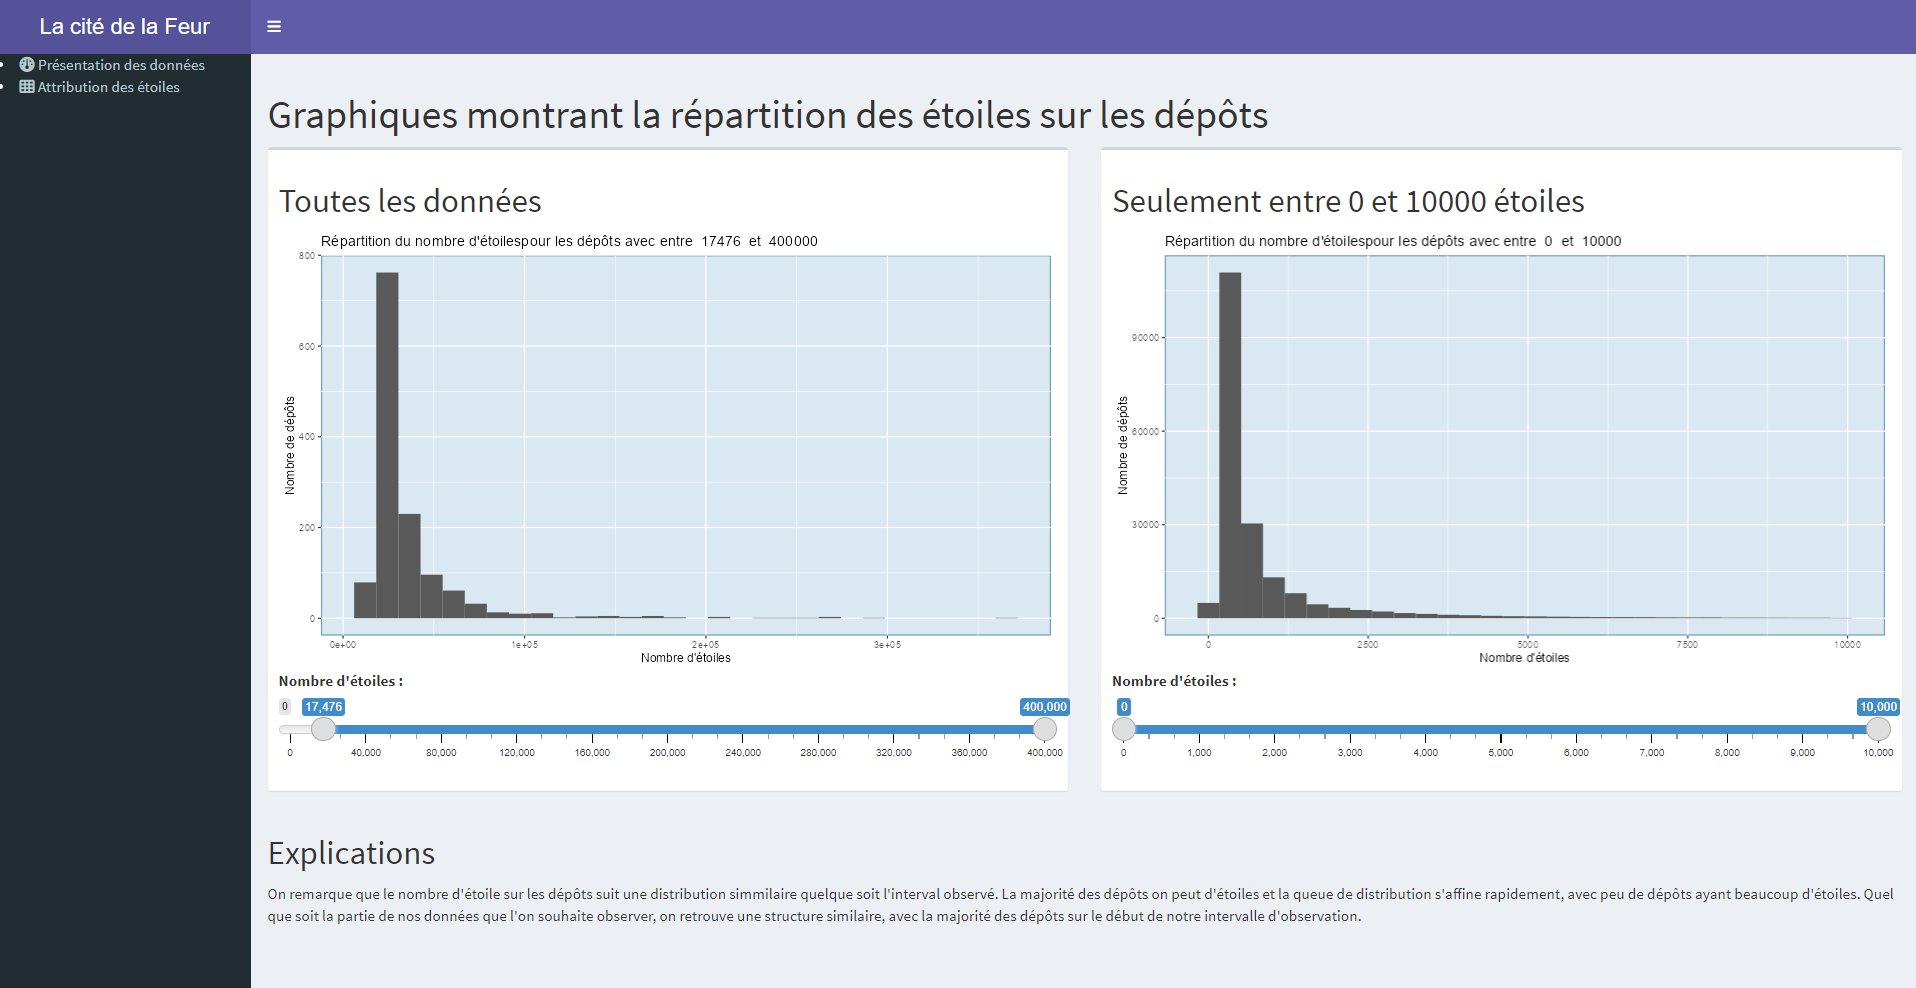
\includegraphics{../img/dashboard_hist_etoiles.png}
\caption{Capture d'écran du dashboard}
\end{figure}

\includegraphics{rapport_files/figure-latex/unnamed-chunk-22-1.pdf}
\includegraphics{rapport_files/figure-latex/unnamed-chunk-22-2.pdf}

\begin{verbatim}
## `stat_bin()` using `bins = 30`. Pick better value with `binwidth`.
\end{verbatim}

\includegraphics{rapport_files/figure-latex/unnamed-chunk-22-3.pdf}

\begin{verbatim}
## `stat_bin()` using `bins = 30`. Pick better value with `binwidth`.
\end{verbatim}

\includegraphics{rapport_files/figure-latex/unnamed-chunk-22-4.pdf}

Quel que soit la partie de nos données que l'on souhaite observer, on
retrouve une structure similaire, avec la majorité des dépôts sur le
début de notre intervalle d'observation.

On comprend avec ce second graphique que la majorité des dépôts ont
moins de 2500 étoiles et quelque uns en ont plus de 5000.

On peut ensuite afficher uniquement les dépôts ayant plus de 10000
étoiles.

\begin{Shaded}
\begin{Highlighting}[]
\FunctionTok{ggplot}\NormalTok{(}\AttributeTok{data =}\NormalTok{ df[df}\SpecialCharTok{$}\NormalTok{stars }\SpecialCharTok{\textgreater{}=} \DecValTok{10000}\NormalTok{,]) }\SpecialCharTok{+}
    \CommentTok{\# Ajoute la géométrie histogramme}
    \FunctionTok{geom\_histogram}\NormalTok{(}\FunctionTok{aes}\NormalTok{(}\AttributeTok{x =}\NormalTok{ stars)) }\SpecialCharTok{+} 
    \FunctionTok{labs}\NormalTok{(}\AttributeTok{x =} \StringTok{"Nombre d\textquotesingle{}étoiles (\textquotesingle{}stars\textquotesingle{}) par classes de 100"}\NormalTok{,}
         \AttributeTok{y =} \StringTok{"Nombre de dépôts"}\NormalTok{,}
         \AttributeTok{title =} \StringTok{"Répartition du nombre d\textquotesingle{}étoiles des dépôts}
\StringTok{         pour les dépôts avec plus de 10000 étoiles"}\NormalTok{)}
\end{Highlighting}
\end{Shaded}

\begin{verbatim}
## `stat_bin()` using `bins = 30`. Pick better value with `binwidth`.
\end{verbatim}

\includegraphics{rapport_files/figure-latex/unnamed-chunk-25-1.pdf} Bien
que l'échelle ne soit plus la même (on atteint \(3\times 10^5\) pour
notre dépôt à 371122 étoiles), on retrouve une distribution très
similaire.

Si l'on se restreint avec les 1000 dépôts avec le plus d'étoiles on a :

\begin{Shaded}
\begin{Highlighting}[]
\CommentTok{\# le dataset df est déjà trié par nombre d\textquotesingle{}étoiles décroissante}
\FunctionTok{ggplot}\NormalTok{(}\AttributeTok{data =}\NormalTok{ df[}\DecValTok{1}\SpecialCharTok{:}\DecValTok{1000}\NormalTok{,]) }\SpecialCharTok{+}
    \CommentTok{\# Ajoute la géométrie histogramme}
    \FunctionTok{geom\_histogram}\NormalTok{(}\FunctionTok{aes}\NormalTok{(}\AttributeTok{x =}\NormalTok{ stars)) }\SpecialCharTok{+} 
    \FunctionTok{labs}\NormalTok{(}\AttributeTok{x =} \StringTok{"Nombre d\textquotesingle{}étoiles (\textquotesingle{}stars\textquotesingle{}) par classes de 100"}\NormalTok{,}
         \AttributeTok{y =} \StringTok{"Nombre de dépôts"}\NormalTok{,}
         \AttributeTok{title =} \StringTok{"Répartition du nombre d\textquotesingle{}étoiles des dépôts}
\StringTok{         pour les dépôts avec plus de 10000 étoiles"}\NormalTok{) }\SpecialCharTok{+}
\NormalTok{  custom\_theme}
\end{Highlighting}
\end{Shaded}

\begin{verbatim}
## `stat_bin()` using `bins = 30`. Pick better value with `binwidth`.
\end{verbatim}

\includegraphics{rapport_files/figure-latex/unnamed-chunk-26-1.pdf}

Il semble que l'on retrouve encore une distribution avec une forme
similaire.

--\textgreater{}

On peut conclure que notre hypothèse de base était la bonne : la
majorité des dépôts ont peu d'étoiles (``peu d'étoile'' relativement à
notre échantillon, soit entre 97 et 1000) et quelque uns arrivent à
monter plus haut, voir pour certains atteindre des centaines de
milliers.

Pour appuyer cette remarque on peut regarder les 10 dépôts ayant le plus
d'étoiles.

\begin{Shaded}
\begin{Highlighting}[]
\FunctionTok{library}\NormalTok{(}\StringTok{"ggrepel"}\NormalTok{)}
\FunctionTok{ggplot}\NormalTok{(}\FunctionTok{arrange}\NormalTok{(df[}\DecValTok{1}\SpecialCharTok{:}\DecValTok{10}\NormalTok{,],stars),}
       \FunctionTok{aes}\NormalTok{(}\AttributeTok{x =} \DecValTok{1}\SpecialCharTok{:}\DecValTok{10}\NormalTok{, }\AttributeTok{y =}\NormalTok{ stars)) }\SpecialCharTok{+}
    \FunctionTok{geom\_point}\NormalTok{() }\SpecialCharTok{+}
    \FunctionTok{geom\_text\_repel}\NormalTok{(}\FunctionTok{aes}\NormalTok{(}\AttributeTok{label =}\NormalTok{ name)) }\SpecialCharTok{+}
    \CommentTok{\# on ajoute une graduation pour ne pas couper le label du 10 élément}
    \FunctionTok{xlim}\NormalTok{(}\DecValTok{0}\NormalTok{,}\DecValTok{11}\NormalTok{) }\SpecialCharTok{+}
    \FunctionTok{labs}\NormalTok{(}\AttributeTok{title =} \StringTok{"Nombre d\textquotesingle{}étoile des 10 projets en ayant le plus}
\StringTok{         sur GitHub"}\NormalTok{,}
         \AttributeTok{x =} \StringTok{" "}\NormalTok{,}
         \AttributeTok{y =} \StringTok{"Nombre d\textquotesingle{}étoiles"}\NormalTok{) }\SpecialCharTok{+}
    \CommentTok{\# améliorer l\textquotesingle{}échelle affichée pour les ordonnés}
    \FunctionTok{scale\_y\_continuous}\NormalTok{(}\AttributeTok{breaks =} \FunctionTok{seq}\NormalTok{(}\DecValTok{200000}\NormalTok{,}\DecValTok{400000}\NormalTok{,}\DecValTok{10000}\NormalTok{)) }\SpecialCharTok{+}
    \CommentTok{\# retire l\textquotesingle{}échelle en abscisse}
    \FunctionTok{theme}\NormalTok{(}\AttributeTok{axis.text.x =} \FunctionTok{element\_blank}\NormalTok{(),}
          \AttributeTok{axis.ticks =} \FunctionTok{element\_blank}\NormalTok{()) }\SpecialCharTok{+}
\NormalTok{  custom\_theme}
\end{Highlighting}
\end{Shaded}

\includegraphics{rapport_files/figure-latex/unnamed-chunk-27-1.pdf}

On remarque immédiatement qu'il y a plus de 100000 étoiles de différence
entre le dépôt \texttt{freeCodeCamp} qui en possède 371122 et le dépôt
\texttt{react} qui en possède 211912.

\begin{Shaded}
\begin{Highlighting}[]
\FunctionTok{sprintf}\NormalTok{(}\StringTok{"Nombre d\textquotesingle{}étoiles de \%s : \%d"}\NormalTok{, df[}\DecValTok{1}\NormalTok{,]}\SpecialCharTok{$}\NormalTok{name, df[}\DecValTok{1}\NormalTok{,]}\SpecialCharTok{$}\NormalTok{stars)}
\end{Highlighting}
\end{Shaded}

\begin{verbatim}
## [1] "Nombre d'étoiles de freeCodeCamp : 371122"
\end{verbatim}

\begin{Shaded}
\begin{Highlighting}[]
\FunctionTok{sprintf}\NormalTok{(}\StringTok{"Nombre d\textquotesingle{}étoiles de \%s : \%d"}\NormalTok{, df[}\DecValTok{10}\NormalTok{,]}\SpecialCharTok{$}\NormalTok{name, df[}\DecValTok{10}\NormalTok{,]}\SpecialCharTok{$}\NormalTok{stars)}
\end{Highlighting}
\end{Shaded}

\begin{verbatim}
## [1] "Nombre d'étoiles de react : 211912"
\end{verbatim}

L'augmentation du nombre d'étoile n'est absolument pas linéaire et
grimper dans le classement de \emph{popularité} est de plus en plus
difficile à mesure que l'on progresse.

Si l'on considère le nombre d'étoile comme une variable aléatoire, on
pourrait essayer d'estimer la loi de cette dernière.

En première approche on peut tester l'hypothèse selon laquelle cette
variable aléatoire suit une loi exponentielle (le plus probable au vu
des histogrammes tracés précédemment).

\begin{Shaded}
\begin{Highlighting}[]
\CommentTok{\# crée une séquence de 1 à 400000}
\NormalTok{s }\OtherTok{\textless{}{-}} \FunctionTok{seq}\NormalTok{(}\DecValTok{0}\NormalTok{,}\DecValTok{400000}\NormalTok{,}\DecValTok{1}\NormalTok{)}
\CommentTok{\# mesure}
\NormalTok{lambda\_mm }\OtherTok{\textless{}{-}} \DecValTok{1}\SpecialCharTok{/}\FunctionTok{mean}\NormalTok{(df}\SpecialCharTok{$}\NormalTok{stars)}
\FunctionTok{ggplot}\NormalTok{() }\SpecialCharTok{+}
  \CommentTok{\# fonction de répartition mesurée}
  \FunctionTok{geom\_line}\NormalTok{(}\FunctionTok{aes}\NormalTok{(}\AttributeTok{x =} \FunctionTok{sort}\NormalTok{(df}\SpecialCharTok{$}\NormalTok{stars, }\AttributeTok{decreasing =} \ConstantTok{FALSE}\NormalTok{), }\AttributeTok{y =} \DecValTok{1}\SpecialCharTok{:}\NormalTok{n}\SpecialCharTok{/}\NormalTok{n)) }\SpecialCharTok{+}
  \CommentTok{\# loi exponentielle avec un paramètre estimé par méthode des moments}
  \CommentTok{\# pour ce jeu de données}
  \FunctionTok{geom\_line}\NormalTok{(}\FunctionTok{aes}\NormalTok{(}\AttributeTok{x =}\NormalTok{ s, }\AttributeTok{y =} \FunctionTok{pexp}\NormalTok{(s, }\AttributeTok{rate =}\NormalTok{ lambda\_mm), }\AttributeTok{color =} \StringTok{\textquotesingle{}red\textquotesingle{}}\NormalTok{)) }\SpecialCharTok{+}
\NormalTok{  custom\_theme}
\end{Highlighting}
\end{Shaded}

\includegraphics{rapport_files/figure-latex/unnamed-chunk-29-1.pdf}

\begin{Shaded}
\begin{Highlighting}[]
\FunctionTok{ggplot}\NormalTok{() }\SpecialCharTok{+}
  \CommentTok{\# fonction de répartition mesurée}
  \FunctionTok{geom\_line}\NormalTok{(}\FunctionTok{aes}\NormalTok{(}\AttributeTok{x =} \FunctionTok{sort}\NormalTok{(df}\SpecialCharTok{$}\NormalTok{stars, }\AttributeTok{decreasing =} \ConstantTok{FALSE}\NormalTok{), }\AttributeTok{y =} \DecValTok{1}\SpecialCharTok{:}\NormalTok{n}\SpecialCharTok{/}\NormalTok{n)) }\SpecialCharTok{+}
  \CommentTok{\# loi exponentielle avec un paramètre estimé par méthode des moments}
  \CommentTok{\# pour ce jeu de données}
  \FunctionTok{geom\_line}\NormalTok{(}\FunctionTok{aes}\NormalTok{(}\AttributeTok{x =}\NormalTok{ s, }\AttributeTok{y =} \FunctionTok{pexp}\NormalTok{(s, }\AttributeTok{rate =}\NormalTok{ lambda\_mm), }\AttributeTok{color =} \StringTok{\textquotesingle{}red\textquotesingle{}}\NormalTok{)) }\SpecialCharTok{+}
  \FunctionTok{xlim}\NormalTok{(}\DecValTok{0}\NormalTok{,}\DecValTok{1000}\NormalTok{) }\SpecialCharTok{+}
\NormalTok{  custom\_theme}
\end{Highlighting}
\end{Shaded}

\begin{verbatim}
## Warning: Removed 41124 rows containing missing values or values outside the scale range
## (`geom_line()`).
\end{verbatim}

\begin{verbatim}
## Warning: Removed 399000 rows containing missing values or values outside the scale range
## (`geom_line()`).
\end{verbatim}

\includegraphics{rapport_files/figure-latex/unnamed-chunk-29-2.pdf}

explication relative à l'estimation de paramètre de lois par
\href{https://fr.wikipedia.org/wiki/M\%C3\%A9thode_des_moments_(statistiques)}{méthode
des moments}

Graphiquement l'approximation par une loi exponentielle n'est pas très
bonne. Il faudrait pousser l'analyse statistique plus loin pour
conclure, ce qui n'est pas l'objet de cette analyse.

Dans l'introduction de ce rapport, nous avions émis l'hypothèse selon
laquelle le nombre d'étoile des dépôt se répartissait selon le principe
de \href{https://fr.wikipedia.org/wiki/Principe_de_Pareto}{Pareto}.

Selon ce principe, 20\% des causes produisent 80\% des effets. Dans
notre cas, cela signifierait que 20\% des dépôts de notre jeu de données
représenteraient 80\% du nombre total d'étoiles.

On peut construire un diagramme de Pareto :

\begin{Shaded}
\begin{Highlighting}[]
\NormalTok{p }\OtherTok{\textless{}{-}} \FunctionTok{ggplot}\NormalTok{() }\SpecialCharTok{+}
    \FunctionTok{geom\_line}\NormalTok{(}\FunctionTok{aes}\NormalTok{(}\AttributeTok{x =}\NormalTok{ (}\DecValTok{1}\SpecialCharTok{:}\NormalTok{n)}\SpecialCharTok{*}\DecValTok{100}\SpecialCharTok{/}\NormalTok{n, }\AttributeTok{y =} \FunctionTok{cumsum}\NormalTok{(df}\SpecialCharTok{$}\NormalTok{stars)}\SpecialCharTok{*}\DecValTok{100}\SpecialCharTok{/}\FunctionTok{sum}\NormalTok{(df}\SpecialCharTok{$}\NormalTok{stars))) }\SpecialCharTok{+}
    \FunctionTok{labs}\NormalTok{(}\AttributeTok{title =} \StringTok{"Diagramme de Pareto du nombre d\textquotesingle{}étoiles en fonction des}
\StringTok{         dépôts"}\NormalTok{,}
         \AttributeTok{x =} \StringTok{"dépôts du jeu de données dans l\textquotesingle{}ordre décroissant du nombre d\textquotesingle{}étoiles, en \%"}\NormalTok{,}
         \AttributeTok{y =} \StringTok{"\% de la somme cumulée du nombre d\textquotesingle{}étoile de notre jeu de données"}\NormalTok{) }\SpecialCharTok{+}
    \FunctionTok{scale\_y\_continuous}\NormalTok{(}\AttributeTok{breaks =} \FunctionTok{seq}\NormalTok{(}\DecValTok{0}\NormalTok{,}\DecValTok{100}\NormalTok{,}\DecValTok{10}\NormalTok{)) }\SpecialCharTok{+}
    \FunctionTok{scale\_x\_continuous}\NormalTok{(}\AttributeTok{breaks =} \FunctionTok{seq}\NormalTok{(}\DecValTok{0}\NormalTok{,}\DecValTok{100}\NormalTok{,}\DecValTok{10}\NormalTok{))}
\NormalTok{p }\SpecialCharTok{+}
    \FunctionTok{geom\_vline}\NormalTok{(}\AttributeTok{xintercept =} \DecValTok{20}\NormalTok{,}
               \AttributeTok{linetype =} \StringTok{"dashed"}\NormalTok{,}
               \AttributeTok{color =} \StringTok{"red"}\NormalTok{) }\SpecialCharTok{+}
    \FunctionTok{geom\_hline}\NormalTok{(}\AttributeTok{yintercept =} \DecValTok{73}\NormalTok{,}
               \AttributeTok{linetype =} \StringTok{"dashed"}\NormalTok{,}
               \AttributeTok{color =} \StringTok{"red"}\NormalTok{) }\SpecialCharTok{+}
\NormalTok{  custom\_theme}
\end{Highlighting}
\end{Shaded}

\includegraphics{rapport_files/figure-latex/unnamed-chunk-30-1.pdf}

Ce diagramme peut se lire ainsi : ``20\% des dépôts (lecture sur l'axe
des abscisses) représentent environ 73\% (lecture sur l'axe des
ordonnés) du nombre total d'étoiles de notre jeu de données''.

Comme sur ce graphique les dépôts sont classés par ordre décroissant
d'étoiles, on peut dire que les 20\% des dépôts ayant le plus d'étoiles
ont à eux seul environ 73\% des étoiles totales attribuées sur GitHub
(avec le biais de sélection dont on a parlé plus haut).

Le principe de Pareto s'applique donc dans une certaine mesure ici.

Si l'on considère le nombre d'étoile d'un dépôt comme un marqueur de sa
``popularité'', on peut ensuite se demander comment expliquer cette
popularité.

On dispose de plusieurs informations conernant les dépôts qui peuvent
nous renseigner :

\begin{itemize}
\tightlist
\item
  les langages utilisés
\item
  les \emph{topics} (les tags associés au dépôt)
\item
  la date de création
\end{itemize}

\subsection{2.3 La date création d'un dépot influence-t-elle sa
popularité
?}\label{la-date-cruxe9ation-dun-duxe9pot-influence-t-elle-sa-popularituxe9}

On peut par exemple penser que plus un dépôt est ancien, plus son nombre
d'étoile est important. C'est un raisonnement plutôt naturel : ce qui
est plus ancien à eu le temps de se faire connaître et donc de gagner en
popularité.

Notre dataset dispose d'un attribut \texttt{createdAt}.

\begin{Shaded}
\begin{Highlighting}[]
\FunctionTok{str}\NormalTok{(df}\SpecialCharTok{$}\NormalTok{createdAt)}
\end{Highlighting}
\end{Shaded}

\begin{verbatim}
##  POSIXct[1:194196], format: "2014-12-24 17:49:19" "2013-10-11 06:50:37" "2019-03-26 07:31:14" ...
\end{verbatim}

Les informations sont stockées dans un format \texttt{POSIXct} qui l'un
des deux formats utilisés pour stocker des dates.

Nous n'avons pas besoin de conserver une précision sur l'heure de
création des dépôts, on peut donc commencer par ne regarder que la date
:

\begin{Shaded}
\begin{Highlighting}[]
\CommentTok{\# On crée une nouvelle colonne au dataset en convertissant la date dans}
\CommentTok{\# un format plus simple : aaaa{-}mm{-}jj}
\NormalTok{df }\OtherTok{\textless{}{-}}\NormalTok{ df }\SpecialCharTok{\%\textgreater{}\%} \FunctionTok{mutate}\NormalTok{(}\AttributeTok{creationDate =} \FunctionTok{as.Date}\NormalTok{(createdAt))}
\end{Highlighting}
\end{Shaded}

On va donc utiliser un
\href{https://datavizcatalogue.com/methods/scatterplot.html}{scatterplot}
pour observer une possible corrélation entre la date de création et le
nombre d'étoiles d'un dépôt.

On utilise directement une échelle logarithmique pour éviter d'avoir un
effet de ``tassement'' des dépôts à cause des différences extrêmes dans
les ordres de grandeur.

Sur ce graphique, les points qui se détachent de la base de points noirs
(coordonnée \(0e+00\) sur l'axe des ordonnés) sont ceux qui ont atteint
un nombre important d'étoiles.

On retrouve notre dépôt \texttt{freeCodeCamp} qui possède le plus
d'étoile en haut au centre :

\begin{Shaded}
\begin{Highlighting}[]
\FunctionTok{ggplot}\NormalTok{(df, }\FunctionTok{aes}\NormalTok{(}\AttributeTok{x =}\NormalTok{ creationDate, }\AttributeTok{y =}\NormalTok{ stars)) }\SpecialCharTok{+}
    \FunctionTok{geom\_point}\NormalTok{(}\AttributeTok{size =} \FloatTok{0.5}\NormalTok{) }\SpecialCharTok{+}
    \FunctionTok{geom\_point}\NormalTok{(}\FunctionTok{aes}\NormalTok{(}\AttributeTok{x =}\NormalTok{ df[df}\SpecialCharTok{$}\NormalTok{name }\SpecialCharTok{==} \StringTok{\textquotesingle{}freeCodeCamp\textquotesingle{}}\NormalTok{,]}\SpecialCharTok{$}\NormalTok{creationDate,}
                   \AttributeTok{y =}\NormalTok{ df[df}\SpecialCharTok{$}\NormalTok{name }\SpecialCharTok{==} \StringTok{\textquotesingle{}freeCodeCamp\textquotesingle{}}\NormalTok{,]}\SpecialCharTok{$}\NormalTok{stars),}
               \AttributeTok{shape =} \DecValTok{1}\NormalTok{,}
               \AttributeTok{size =} \DecValTok{6}\NormalTok{,}
               \AttributeTok{color =} \StringTok{\textquotesingle{}red\textquotesingle{}}\NormalTok{) }\SpecialCharTok{+} 
    \FunctionTok{scale\_x\_date}\NormalTok{(}\AttributeTok{breaks =}\NormalTok{ datebreaks) }\SpecialCharTok{+}
    \CommentTok{\# pour afficher les dates en biais}
    \FunctionTok{theme}\NormalTok{(}\AttributeTok{axis.text.x =} \FunctionTok{element\_text}\NormalTok{(}\AttributeTok{angle =} \DecValTok{30}\NormalTok{, }\AttributeTok{hjust =} \DecValTok{1}\NormalTok{)) }\SpecialCharTok{+}
    \FunctionTok{labs}\NormalTok{(}\AttributeTok{title =} \StringTok{"Nombre d\textquotesingle{}étoiles en fonction de la date de}
\StringTok{         création des dépôts"}\NormalTok{,}
         \AttributeTok{x =} \StringTok{"Date de création des dépôts"}\NormalTok{,}
         \AttributeTok{y =} \StringTok{"Nombre d\textquotesingle{}étoile des dépôts"}\NormalTok{)}
\end{Highlighting}
\end{Shaded}

\begin{verbatim}
## Warning in geom_point(aes(x = df[df$name == "freeCodeCamp", ]$creationDate, : All aesthetics have length 1, but the data has 194196 rows.
## i Did you mean to use `annotate()`?
\end{verbatim}

\includegraphics{rapport_files/figure-latex/unnamed-chunk-34-1.pdf}

Attention, encore une fois à l'échelle utilisée dans ce graphique :
comme nous avons une très forte disparité entre le nombre d'étoile des
dépôts, nous affichons en même temps des dépôts avec un nombre d'étoile
dans les centaine (\(10^2\)) et des dépôts avec des centaines de
milliers d'étoiles (\(10^5\)).

Ce graphique nous montre très clairement que la date de création du
dépôt n'influence en rien la popularité de ces derniers : on trouve des
dépôts aujourd'hui populaire créés dans les premières années de GitHub
(2009-2010), comme des dépôt populaire très récents (2023).

Si l'on utilise une échelle logarithmique pour le nombre d'étoile on
s'en rend mieux compte que les dépôts ``populaires

\begin{Shaded}
\begin{Highlighting}[]
\CommentTok{\# on crée les graduations en abscisse pour faciliter la lecture}
\NormalTok{datebreaks }\OtherTok{\textless{}{-}} \FunctionTok{seq}\NormalTok{(}\FunctionTok{as.Date}\NormalTok{(}\StringTok{"2009{-}01{-}01"}\NormalTok{), }\FunctionTok{as.Date}\NormalTok{(}\StringTok{"2024{-}01{-}01"}\NormalTok{), }\AttributeTok{by =} \StringTok{"1 year"}\NormalTok{)}

\FunctionTok{ggplot}\NormalTok{(df, }\FunctionTok{aes}\NormalTok{(}\AttributeTok{x =}\NormalTok{ creationDate, }\AttributeTok{y =}\NormalTok{ stars)) }\SpecialCharTok{+}
    \FunctionTok{geom\_point}\NormalTok{(}\AttributeTok{size =} \FloatTok{0.5}\NormalTok{) }\SpecialCharTok{+}
    \FunctionTok{scale\_y\_log10}\NormalTok{() }\SpecialCharTok{+}
    \FunctionTok{scale\_x\_date}\NormalTok{(}\AttributeTok{breaks =}\NormalTok{ datebreaks) }\SpecialCharTok{+}
    \CommentTok{\# pour afficher les dates en biais}
    \FunctionTok{theme}\NormalTok{(}\AttributeTok{axis.text.x =} \FunctionTok{element\_text}\NormalTok{(}\AttributeTok{angle =} \DecValTok{30}\NormalTok{, }\AttributeTok{hjust =} \DecValTok{1}\NormalTok{)) }\SpecialCharTok{+}
    \FunctionTok{labs}\NormalTok{(}\AttributeTok{title =} \StringTok{"Nombre d\textquotesingle{}étoiles en fonction de la date de}
\StringTok{         création des dépôts"}\NormalTok{,}
         \AttributeTok{x =} \StringTok{"Date de création des dépôts"}\NormalTok{,}
         \AttributeTok{y =} \StringTok{"Nombre d\textquotesingle{}étoile des dépôts"}\NormalTok{,}
         \AttributeTok{subtitle =} \StringTok{"Le nombre d\textquotesingle{}étoile est représenté par une échelle}
\StringTok{         logarithmique"}\NormalTok{)}
\end{Highlighting}
\end{Shaded}

\includegraphics{rapport_files/figure-latex/unnamed-chunk-35-1.pdf}

On peut se convaincre en affichant la moyenne des étoiles des dépôts
pour chaque année création (la moyenne pour les dépôts créés entre 2009
et 2010, pour ceux créés entre 2010 et 2011, etc.).

\begin{Shaded}
\begin{Highlighting}[]
\CommentTok{\# On calcul la moyenne du nombre d\textquotesingle{}étoiles des dépôt en fonction de leurs}
\CommentTok{\# \# date de création en divisant en années}
\NormalTok{separation\_annees }\OtherTok{\textless{}{-}} \FunctionTok{paste}\NormalTok{(}\DecValTok{2009}\SpecialCharTok{:}\DecValTok{2023}\NormalTok{,}\StringTok{"{-}01{-}01"}\NormalTok{,}\AttributeTok{sep=}\StringTok{""}\NormalTok{)}
\NormalTok{separation\_annees[}\FunctionTok{length}\NormalTok{(separation\_annees)}\SpecialCharTok{+}\DecValTok{1}\NormalTok{] }\OtherTok{\textless{}{-}} \FunctionTok{as.character}\NormalTok{(}\FunctionTok{max}\NormalTok{(df}\SpecialCharTok{$}\NormalTok{creationDate))}
\NormalTok{separation\_annees[}\FunctionTok{length}\NormalTok{(separation\_annees)] }\OtherTok{\textless{}{-}} \FunctionTok{as.character}\NormalTok{(}\FunctionTok{as.Date}\NormalTok{(separation\_annees[}\FunctionTok{length}\NormalTok{(separation\_annees)]) }\SpecialCharTok{+} \DecValTok{1}\NormalTok{)}
\CommentTok{\# nbr = 0}
\NormalTok{mean\_stars\_by\_year }\OtherTok{\textless{}{-}} \FunctionTok{c}\NormalTok{()}
\ControlFlowTok{for}\NormalTok{ (i }\ControlFlowTok{in} \DecValTok{2}\SpecialCharTok{:}\FunctionTok{length}\NormalTok{(separation\_annees)) \{}
    \CommentTok{\# nbr = nbr + dim(df[df$creationDate \textless{} separation\_annees[i] \&}
    \CommentTok{\#                   df$creationDate \textgreater{}= separation\_annees[i{-}1],])[1]}
    \CommentTok{\# Pour vérifier le nombre d\textquotesingle{}éléments comptés}
    
\NormalTok{    mean\_stars\_by\_year }\OtherTok{\textless{}{-}} \FunctionTok{c}\NormalTok{(}
\NormalTok{        mean\_stars\_by\_year,}
        \FunctionTok{mean}\NormalTok{(df[df}\SpecialCharTok{$}\NormalTok{creationDate }\SpecialCharTok{\textless{}}\NormalTok{ separation\_annees[i] }\SpecialCharTok{\&}
\NormalTok{           df}\SpecialCharTok{$}\NormalTok{creationDate }\SpecialCharTok{\textgreater{}=}\NormalTok{ separation\_annees[i}\DecValTok{{-}1}\NormalTok{],]}\SpecialCharTok{$}\NormalTok{stars)}
\NormalTok{    )}
\NormalTok{\}}
\end{Highlighting}
\end{Shaded}

\begin{Shaded}
\begin{Highlighting}[]
\FunctionTok{ggplot}\NormalTok{() }\SpecialCharTok{+}
    \FunctionTok{geom\_point}\NormalTok{(}\FunctionTok{aes}\NormalTok{(}\AttributeTok{x =}\NormalTok{ df}\SpecialCharTok{$}\NormalTok{creationDate, }\AttributeTok{y =}\NormalTok{ df}\SpecialCharTok{$}\NormalTok{stars), }\AttributeTok{size =} \FloatTok{0.5}\NormalTok{) }\SpecialCharTok{+}
    \FunctionTok{geom\_line}\NormalTok{(}\FunctionTok{aes}\NormalTok{(}\AttributeTok{x =} \FunctionTok{as.Date}\NormalTok{(separation\_annees[}\DecValTok{1}\SpecialCharTok{:}\NormalTok{(}\FunctionTok{length}\NormalTok{(separation\_annees)}\SpecialCharTok{{-}}\DecValTok{1}\NormalTok{)]),}
                  \AttributeTok{y =}\NormalTok{ mean\_stars\_by\_year), }\AttributeTok{color =} \StringTok{"red"}\NormalTok{) }\SpecialCharTok{+}
    \FunctionTok{scale\_y\_log10}\NormalTok{() }\SpecialCharTok{+}
    \FunctionTok{scale\_x\_date}\NormalTok{(}\AttributeTok{breaks =}\NormalTok{ datebreaks) }\SpecialCharTok{+}
    \CommentTok{\# pour afficher les dates en biais}
    \FunctionTok{theme}\NormalTok{(}\AttributeTok{axis.text.x =} \FunctionTok{element\_text}\NormalTok{(}\AttributeTok{angle =} \DecValTok{30}\NormalTok{, }\AttributeTok{hjust =} \DecValTok{1}\NormalTok{)) }\SpecialCharTok{+}
    \FunctionTok{labs}\NormalTok{(}\AttributeTok{title =} \StringTok{"Nombre d\textquotesingle{}étoiles en fonction de la date de}
\StringTok{         création des dépôts"}\NormalTok{,}
         \AttributeTok{x =} \StringTok{"Date de création des dépôts"}\NormalTok{,}
         \AttributeTok{y =} \StringTok{"Nombre d\textquotesingle{}étoile des dépôts"}\NormalTok{,}
         \AttributeTok{subtitle =} \StringTok{"Le nombre d\textquotesingle{}étoile est représenté par une échelle}
\StringTok{         logarithmique"}\NormalTok{)}
\end{Highlighting}
\end{Shaded}

\includegraphics{rapport_files/figure-latex/unnamed-chunk-37-1.pdf}

On voit bien que la moyenne reste relativement stable. On note une
légère hausse en 2022 qui peut traduire une hausse de popularité de la
plateforme.

Le 25 janvier 2023, GitHub annonçait avoir atteint les
\href{https://github.blog/2023-01-25-100-million-developers-and-counting/}{100
millions d'utilisateurs}.

On peut donc voir dans notre graphique un début d'une augmentation
d'utlisateurs actifs sur la plateforme, sans pouvoir le confirmer.

--\textgreater{}

On ajoute aussi au graphique la moyenne des étoiles des dépôts pour
chaque année création (la moyenne pour les dépôts créés entre 2009 et
2010, pour ceux créés entre 2010 et 2011, etc.)

\begin{Shaded}
\begin{Highlighting}[]
\CommentTok{\# On calcul la moyenne du nombre d\textquotesingle{}étoiles des dépôt en fonction de leurs}
\CommentTok{\# \# date de création en divisant en années}
\NormalTok{separation\_annees }\OtherTok{\textless{}{-}} \FunctionTok{paste}\NormalTok{(}\DecValTok{2009}\SpecialCharTok{:}\DecValTok{2023}\NormalTok{,}\StringTok{"{-}01{-}01"}\NormalTok{,}\AttributeTok{sep=}\StringTok{""}\NormalTok{)}
\NormalTok{separation\_annees[}\FunctionTok{length}\NormalTok{(separation\_annees)}\SpecialCharTok{+}\DecValTok{1}\NormalTok{] }\OtherTok{\textless{}{-}} \FunctionTok{as.character}\NormalTok{(}\FunctionTok{max}\NormalTok{(df}\SpecialCharTok{$}\NormalTok{creationDate))}
\NormalTok{separation\_annees[}\FunctionTok{length}\NormalTok{(separation\_annees)] }\OtherTok{\textless{}{-}} \FunctionTok{as.character}\NormalTok{(}\FunctionTok{as.Date}\NormalTok{(separation\_annees[}\FunctionTok{length}\NormalTok{(separation\_annees)]) }\SpecialCharTok{+} \DecValTok{1}\NormalTok{)}
\CommentTok{\# nbr = 0}
\NormalTok{mean\_stars\_by\_year }\OtherTok{\textless{}{-}} \FunctionTok{c}\NormalTok{()}
\ControlFlowTok{for}\NormalTok{ (i }\ControlFlowTok{in} \DecValTok{2}\SpecialCharTok{:}\FunctionTok{length}\NormalTok{(separation\_annees)) \{}
    \CommentTok{\# nbr = nbr + dim(df[df$creationDate \textless{} separation\_annees[i] \&}
    \CommentTok{\#                   df$creationDate \textgreater{}= separation\_annees[i{-}1],])[1]}
    \CommentTok{\# Pour vérifier le nombre d\textquotesingle{}éléments comptés}
    
\NormalTok{    mean\_stars\_by\_year }\OtherTok{\textless{}{-}} \FunctionTok{c}\NormalTok{(}
\NormalTok{        mean\_stars\_by\_year,}
        \FunctionTok{mean}\NormalTok{(df[df}\SpecialCharTok{$}\NormalTok{creationDate }\SpecialCharTok{\textless{}}\NormalTok{ separation\_annees[i] }\SpecialCharTok{\&}
\NormalTok{           df}\SpecialCharTok{$}\NormalTok{creationDate }\SpecialCharTok{\textgreater{}=}\NormalTok{ separation\_annees[i}\DecValTok{{-}1}\NormalTok{],]}\SpecialCharTok{$}\NormalTok{stars)}
\NormalTok{    )}
\NormalTok{\}}
\end{Highlighting}
\end{Shaded}

\begin{Shaded}
\begin{Highlighting}[]
\NormalTok{datebreaks }\OtherTok{\textless{}{-}} \FunctionTok{seq}\NormalTok{(}\FunctionTok{as.Date}\NormalTok{(}\StringTok{"2009{-}01{-}01"}\NormalTok{), }\FunctionTok{as.Date}\NormalTok{(}\StringTok{"2024{-}01{-}01"}\NormalTok{), }\AttributeTok{by =} \StringTok{"1 year"}\NormalTok{)}
\FunctionTok{ggplot}\NormalTok{() }\SpecialCharTok{+}
  \FunctionTok{geom\_point}\NormalTok{(}\FunctionTok{aes}\NormalTok{(}\AttributeTok{x =}\NormalTok{ df[df}\SpecialCharTok{$}\NormalTok{stars }\SpecialCharTok{\textgreater{}} \DecValTok{130}\NormalTok{,]}\SpecialCharTok{$}\NormalTok{creationDate,}
                 \AttributeTok{y =}\NormalTok{ df[df}\SpecialCharTok{$}\NormalTok{stars }\SpecialCharTok{\textgreater{}} \DecValTok{130}\NormalTok{,]}\SpecialCharTok{$}\NormalTok{stars), }\AttributeTok{size =} \FloatTok{0.5}\NormalTok{) }\SpecialCharTok{+}
  \FunctionTok{geom\_point}\NormalTok{(}\FunctionTok{aes}\NormalTok{(}\AttributeTok{x =}\NormalTok{ df[df}\SpecialCharTok{$}\NormalTok{name }\SpecialCharTok{==} \StringTok{\textquotesingle{}freeCodeCamp\textquotesingle{}}\NormalTok{,]}\SpecialCharTok{$}\NormalTok{creationDate,}
                 \AttributeTok{y =}\NormalTok{ df[df}\SpecialCharTok{$}\NormalTok{name }\SpecialCharTok{==} \StringTok{\textquotesingle{}freeCodeCamp\textquotesingle{}}\NormalTok{,]}\SpecialCharTok{$}\NormalTok{stars),}
             \AttributeTok{shape =} \DecValTok{1}\NormalTok{,}
             \AttributeTok{size =} \DecValTok{6}\NormalTok{,}
             \AttributeTok{color =} \StringTok{\textquotesingle{}red\textquotesingle{}}\NormalTok{) }\SpecialCharTok{+}
  \FunctionTok{geom\_line}\NormalTok{(}\FunctionTok{aes}\NormalTok{(}\AttributeTok{x =} \FunctionTok{as.Date}\NormalTok{(separation\_annees[}\DecValTok{1}\SpecialCharTok{:}\NormalTok{(}\FunctionTok{length}\NormalTok{(separation\_annees)}\SpecialCharTok{{-}}\DecValTok{1}\NormalTok{)]),}
                \AttributeTok{y =}\NormalTok{ mean\_stars\_by\_year), }\AttributeTok{color =} \StringTok{"red"}\NormalTok{) }\SpecialCharTok{+}
  \FunctionTok{scale\_y\_log10}\NormalTok{() }\SpecialCharTok{+}
  \FunctionTok{scale\_x\_date}\NormalTok{(}\AttributeTok{breaks =}\NormalTok{ datebreaks) }\SpecialCharTok{+}
  \CommentTok{\# pour afficher les dates en biais}
  \FunctionTok{theme}\NormalTok{(}\AttributeTok{axis.text.x =} \FunctionTok{element\_text}\NormalTok{(}\AttributeTok{angle =} \DecValTok{30}\NormalTok{, }\AttributeTok{hjust =} \DecValTok{1}\NormalTok{)) }\SpecialCharTok{+}
  \FunctionTok{labs}\NormalTok{(}\AttributeTok{title =} \StringTok{"Nombre d\textquotesingle{}étoiles en fonction de la date de}
\StringTok{         création des dépôts"}\NormalTok{,}
       \AttributeTok{x =} \StringTok{"Date de création des dépôts"}\NormalTok{,}
       \AttributeTok{y =} \StringTok{"Nombre d\textquotesingle{}étoile des dépôts"}\NormalTok{,}
       \AttributeTok{subtitle =} \StringTok{"Le nombre d\textquotesingle{}étoile est représenté par une échelle}
\StringTok{         logarithmique"}\NormalTok{) }\SpecialCharTok{+}
\NormalTok{  custom\_theme}
\end{Highlighting}
\end{Shaded}

\includegraphics{rapport_files/figure-latex/unnamed-chunk-39-1.pdf}

\begin{Shaded}
\begin{Highlighting}[]
\CommentTok{\# Le lecteur averti aura remarqué que dans cette représentation, nous avons}
\CommentTok{\# retiré les dépôts ayant moins de 130 étoiles.}
\CommentTok{\# ces derniers perturbent la représentation graphique en ajoutant une ligne }
\CommentTok{\# continue en bas du nuage du point pour les dates de 2009 à 2015}
\CommentTok{\# ce qui perturbe la représentation graphique.}
\CommentTok{\# Les retirer n\textquotesingle{}enlève en rien les conclusion faite sur ce graphique.}
\CommentTok{\# et participe uniquement au confort de lecture.}
\end{Highlighting}
\end{Shaded}

L'échelle logarithmique rendant plus difficile l'interprétation du
graphique, nous avons entouré le dépôt \texttt{freeCodeCamp} en rouge.
Ce dépôt qui possède le plus d'étoile a été crée en 2015 et l'échelle
logarithmique le rapproche du reste des dépôts dans le représentation
graphique.

Ce graphique nous montre très clairement que la date de création du
dépôt n'influence en rien la popularité de ces derniers : on trouve des
dépôts aujourd'hui populaire créés dans les premières années de GitHub
(2009-2010), comme des dépôt populaire très récents (2023).

On voit bien que la moyenne reste relativement stable. On note une
légère hausse en 2022 qui peut traduire une hausse de popularité de la
plateforme.

Le 25 janvier 2023, GitHub annonçait avoir atteint les
\href{https://github.blog/2023-01-25-100-million-developers-and-counting/}{100
millions d'utilisateurs}.

On peut donc voir dans notre graphique un début d'une augmentation
d'utilisateurs actifs sur la plateforme, sans pouvoir le confirmer.

\subsection{\texorpdfstring{2.4 Existe-il un lien entre le nombre
d'étoile et le nombre de de \texttt{watchers}
?}{2.4 Existe-il un lien entre le nombre d'étoile et le nombre de de watchers ?}}\label{existe-il-un-lien-entre-le-nombre-duxe9toile-et-le-nombre-de-de-watchers}

Comme évoqué dans la présentation du jeu de données, nous disposons
d'autres indicateurs de ``popularité''. L'un deux, nommé
\texttt{watchers} dans le dataset, indique combien de personne
``suivent'' un dépôt.

Si l'on reprend la métaphore d'un réseau social : un utlisateur peu
\emph{liker} un dépôt qu'il apprécie (ajoute une étoile \emph{stars})
mais il peut également \emph{follow} le dépôt pour être mit au courant
des évolutions.

On peut supposer qu'un dépôt ayant beaucoup d'étoiles aura aussi
beaucoup de \emph{watchers} qui souhaitent être informé des évolutions.

On va donc confirmer ou non cette hypothèse à l'aide d'un
\href{https://datavizcatalogue.com/methods/scatterplot.html}{scatterplot}.

\begin{Shaded}
\begin{Highlighting}[]
\FunctionTok{ggplot}\NormalTok{(df, }\FunctionTok{aes}\NormalTok{(}\AttributeTok{x =}\NormalTok{ stars, }\AttributeTok{y =}\NormalTok{ watchers)) }\SpecialCharTok{+}
  \FunctionTok{geom\_point}\NormalTok{() }\SpecialCharTok{+}
  \FunctionTok{geom\_smooth}\NormalTok{() }\SpecialCharTok{+}
  \FunctionTok{labs}\NormalTok{(}\AttributeTok{x =} \StringTok{"Nombre d\textquotesingle{}étoile des dépôts"}\NormalTok{,}
       \AttributeTok{y =} \StringTok{"Nombre de watchers des dépôts"}\NormalTok{,}
       \AttributeTok{title =} \StringTok{"Nuage de point entre les stars et watchers des dépôts"}\NormalTok{) }\SpecialCharTok{+}
\NormalTok{  custom\_theme}
\end{Highlighting}
\end{Shaded}

\begin{verbatim}
## `geom_smooth()` using method = 'gam' and formula = 'y ~ s(x, bs = "cs")'
\end{verbatim}

\includegraphics{rapport_files/figure-latex/unnamed-chunk-40-1.pdf}

Tel quel le graphique n'est pas exploitable à cause de la très grandes
disparités dans les valeurs de \texttt{stars} qui vient ``tasser'' la
très grande majorité des points dans le coin infénieur gauche
(``faibles'' valeurs de \texttt{stars} et faibles valeurs de
\texttt{watchers})

Nous avons réalisé ce même graphique en utilisant Tableau :

\begin{Shaded}
\begin{Highlighting}[]
\DataTypeTok{\textless{}}\KeywordTok{figure}\DataTypeTok{\textgreater{}}
  \DataTypeTok{\textless{}}\KeywordTok{img}\OtherTok{ src}\OperatorTok{=}\StringTok{"../img/nuage1.png"}\OtherTok{ alt}\OperatorTok{=}\StringTok{"Capture d\textquotesingle{}écran de Tableau"}\OtherTok{ }\DataTypeTok{/\textgreater{}}
  \DataTypeTok{\textless{}}\KeywordTok{figcaption}\DataTypeTok{\textgreater{}}\NormalTok{Capture d\textquotesingle{}écran de Tableau}\DataTypeTok{\textless{}/}\KeywordTok{figcaption}\DataTypeTok{\textgreater{}}
\DataTypeTok{\textless{}/}\KeywordTok{figure}\DataTypeTok{\textgreater{}}
\end{Highlighting}
\end{Shaded}

\begin{figure}
\centering
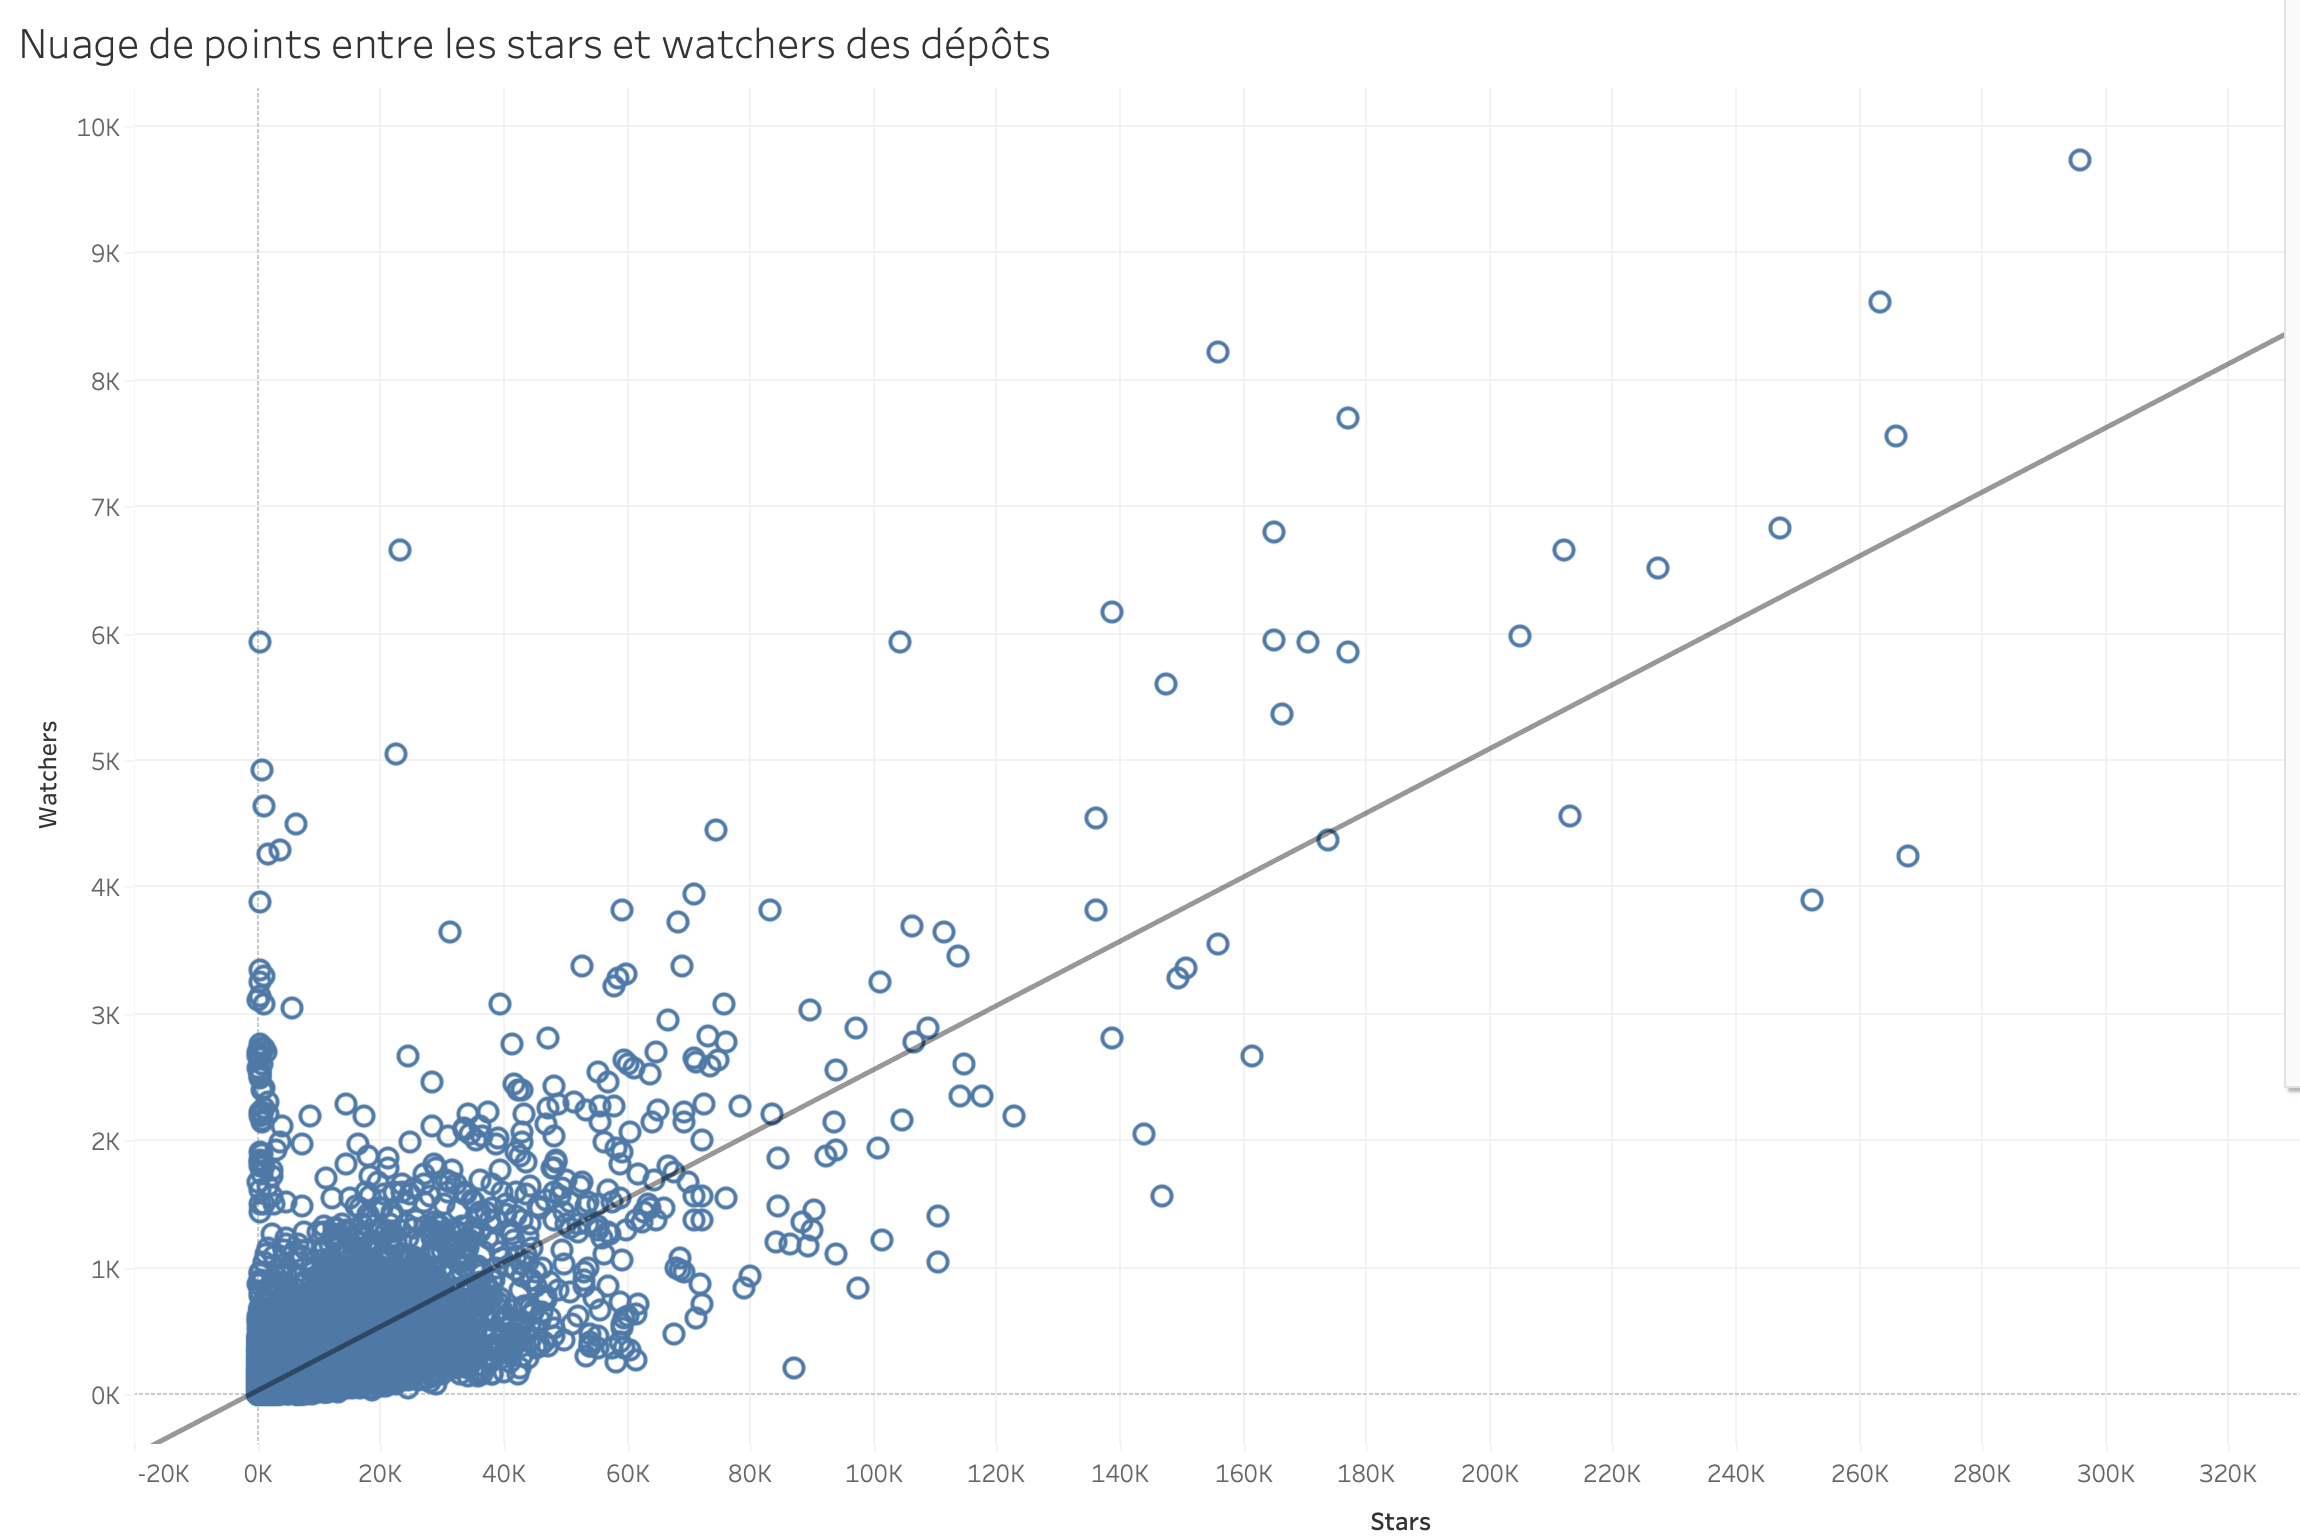
\includegraphics{../img/nuage1.png}
\caption{Capture d'écran de Tableau}
\end{figure}

On peut commencer par tracer le même graphique en retirant tous les
dépôts possédant moins de 10000 étoiles.

\begin{Shaded}
\begin{Highlighting}[]
\FunctionTok{ggplot}\NormalTok{() }\SpecialCharTok{+}
  \FunctionTok{geom\_point}\NormalTok{(}\FunctionTok{aes}\NormalTok{(}\AttributeTok{x =}\NormalTok{ df[df}\SpecialCharTok{$}\NormalTok{stars }\SpecialCharTok{\textless{}=} \DecValTok{10000}\NormalTok{,]}\SpecialCharTok{$}\NormalTok{stars,}
                 \AttributeTok{y =}\NormalTok{ df[df}\SpecialCharTok{$}\NormalTok{stars }\SpecialCharTok{\textless{}=} \DecValTok{10000}\NormalTok{,]}\SpecialCharTok{$}\NormalTok{watchers)) }\SpecialCharTok{+}
  \FunctionTok{geom\_smooth}\NormalTok{(}\FunctionTok{aes}\NormalTok{(}\AttributeTok{x =}\NormalTok{ df[df}\SpecialCharTok{$}\NormalTok{stars }\SpecialCharTok{\textless{}=} \DecValTok{10000}\NormalTok{,]}\SpecialCharTok{$}\NormalTok{stars,}
                 \AttributeTok{y =}\NormalTok{ df[df}\SpecialCharTok{$}\NormalTok{stars }\SpecialCharTok{\textless{}=} \DecValTok{10000}\NormalTok{,]}\SpecialCharTok{$}\NormalTok{watchers)) }\SpecialCharTok{+}
  \FunctionTok{geom\_point}\NormalTok{(}\FunctionTok{aes}\NormalTok{(}\AttributeTok{x =}\NormalTok{ df[df}\SpecialCharTok{$}\NormalTok{stars }\SpecialCharTok{\textless{}=}\NormalTok{ df}\SpecialCharTok{$}\NormalTok{watchers,]}\SpecialCharTok{$}\NormalTok{stars,}
                 \AttributeTok{y =}\NormalTok{ df[df}\SpecialCharTok{$}\NormalTok{stars }\SpecialCharTok{\textless{}=}\NormalTok{ df}\SpecialCharTok{$}\NormalTok{watchers,]}\SpecialCharTok{$}\NormalTok{watchers),}
             \AttributeTok{color =} \StringTok{\textquotesingle{}red\textquotesingle{}}\NormalTok{) }\SpecialCharTok{+}
  \FunctionTok{labs}\NormalTok{(}\AttributeTok{x =} \StringTok{"Nombre d\textquotesingle{}étoile des dépôts"}\NormalTok{,}
       \AttributeTok{y =} \StringTok{"Nombre de watchers des dépôts"}\NormalTok{,}
       \AttributeTok{title =} \StringTok{"Nuage de point entre les stars et watchers des dépôts }
\StringTok{       pour les dépôts de moins de 10000 étoiles."}\NormalTok{,}
       \AttributeTok{subtitle =} \StringTok{"En rouge les dépôts avec moins d\textquotesingle{}étoiles que de watchers"}\NormalTok{) }\SpecialCharTok{+}
\NormalTok{  custom\_theme}
\end{Highlighting}
\end{Shaded}

\begin{verbatim}
## `geom_smooth()` using method = 'gam' and formula = 'y ~ s(x, bs = "cs")'
\end{verbatim}

\includegraphics{rapport_files/figure-latex/unnamed-chunk-41-1.pdf}

Contrairement à notre hypothèse de base, il semble que le nombre de
\texttt{watchers} n'évolue que très peu quelque soit le nombre d'étoile
attribué au dépôt.

Nous avons réalisé ce même graphique en utilisant Tableau :

\begin{Shaded}
\begin{Highlighting}[]
\DataTypeTok{\textless{}}\KeywordTok{figure}\DataTypeTok{\textgreater{}}
  \DataTypeTok{\textless{}}\KeywordTok{img}\OtherTok{ src}\OperatorTok{=}\StringTok{"../img/nuage2.png"}\OtherTok{ alt}\OperatorTok{=}\StringTok{"Capture d\textquotesingle{}écran de Tableau"}\OtherTok{ }\DataTypeTok{/\textgreater{}}
  \DataTypeTok{\textless{}}\KeywordTok{figcaption}\DataTypeTok{\textgreater{}}\NormalTok{Capture d\textquotesingle{}écran de Tableau}\DataTypeTok{\textless{}/}\KeywordTok{figcaption}\DataTypeTok{\textgreater{}}
\DataTypeTok{\textless{}/}\KeywordTok{figure}\DataTypeTok{\textgreater{}}
\end{Highlighting}
\end{Shaded}

\begin{figure}
\centering
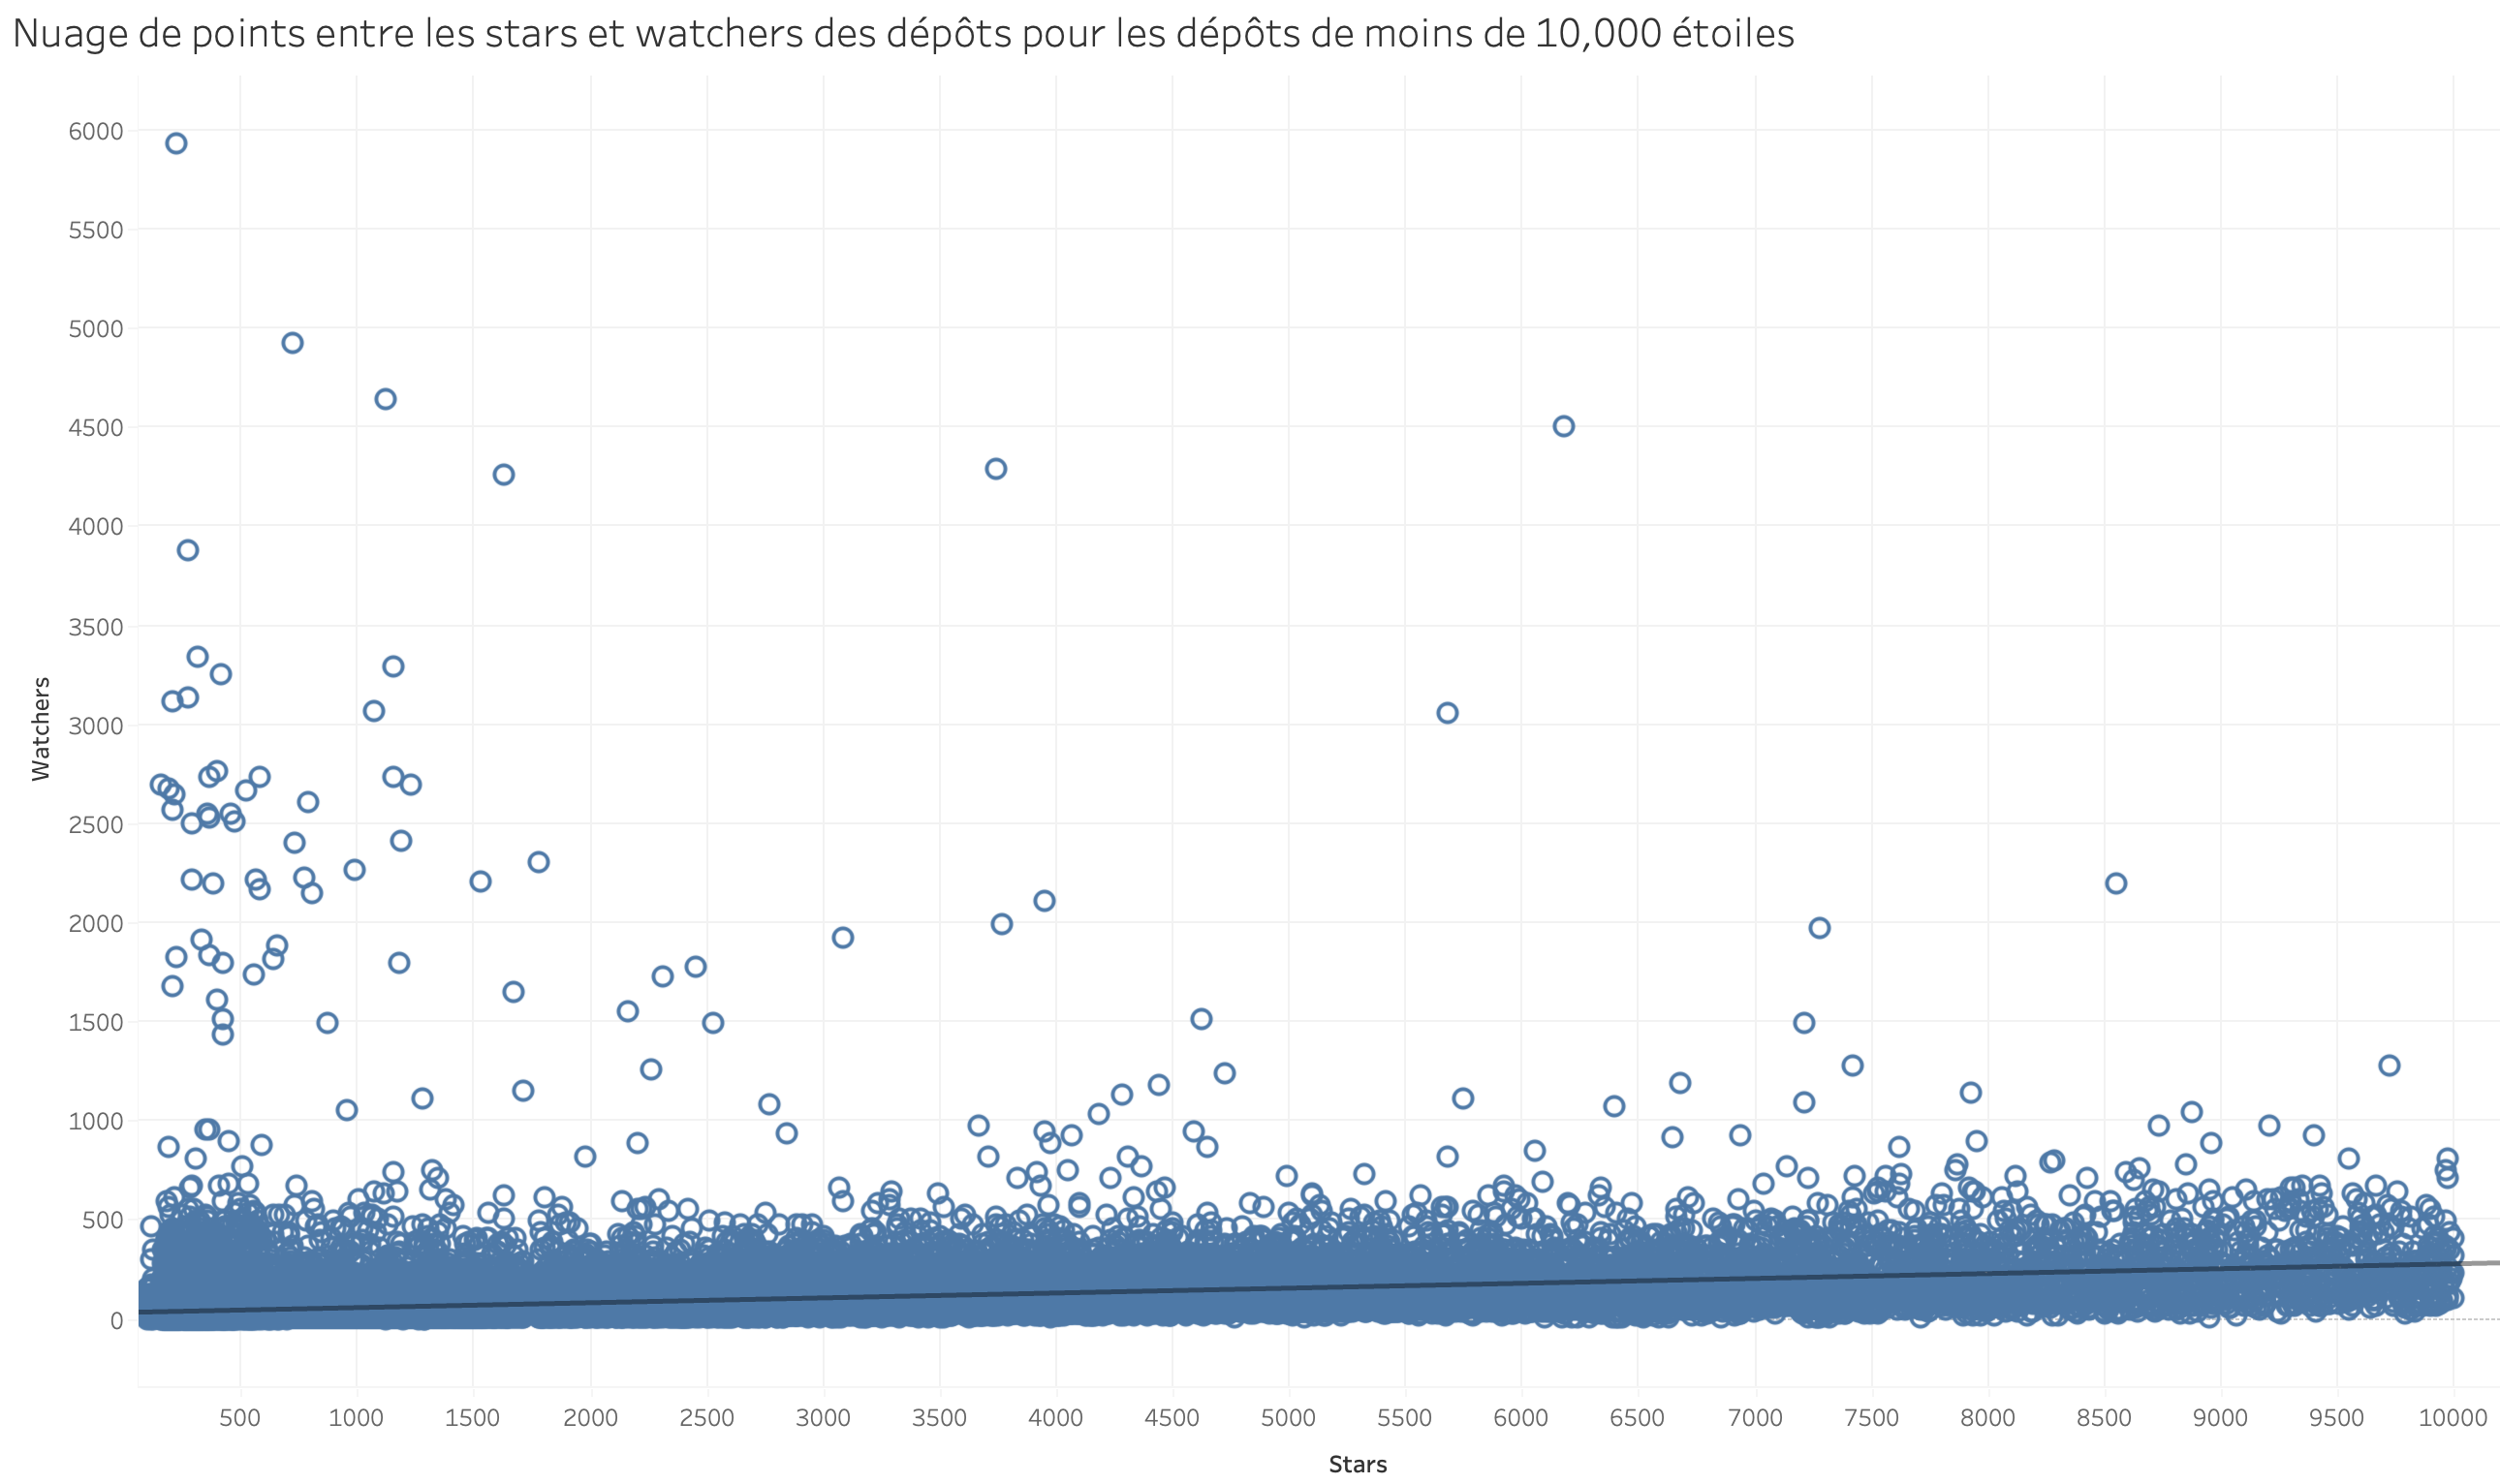
\includegraphics{../img/nuage2.png}
\caption{Capture d'écran de Tableau}
\end{figure}

On observe quelque dépôts qui sortent du lot (valeurs abérantes) qui
possèdent plus de \texttt{watchers} que de \texttt{stars} (ce qui va à
l'encontre de la très large majorité des dépôts). Nous les avons affiché
en rouge sur le précédent graphique.

Si l'on observe les noms de ces dépôts :

\begin{Shaded}
\begin{Highlighting}[]
\CommentTok{\# Liste complète}
\CommentTok{\# df[df$stars \textless{}= df$watchers,]$nameWithOwner}
\FunctionTok{head}\NormalTok{(df[df}\SpecialCharTok{$}\NormalTok{stars }\SpecialCharTok{\textless{}=}\NormalTok{ df}\SpecialCharTok{$}\NormalTok{watchers,]}\SpecialCharTok{$}\NormalTok{nameWithOwner)}
\end{Highlighting}
\end{Shaded}

\begin{verbatim}
## [1] "Azure/azure-powershell"                  
## [2] "microsoft/code-with-engineering-playbook"
## [3] "aspnet/Announcements"                    
## [4] "uber/okbuck"                             
## [5] "Azure/azureml-examples"                  
## [6] "Azure/azure-sdk-for-node"
\end{verbatim}

On remarque qu'il s'agit surtout de dépôt publics créés par des grandes
entreprises comme Microsoft (les produits Azure entre autre), Uber,
Netflix, Shopify, etc.

On peut donc supposer que ces dépôt abritent le code source de
programmes ré-utilisés par de nombreux développeurs (tel que des API ou
des SDK : software development kit).

Les entreprises ou développeurs utilisant ces programmes doivent donc
souhaiter être tenu a jours des évolutions (ce sont des
\texttt{watchers}) sans pour autant \emph{liker} le dépôt (sans prendre
le temps de le faire).

On remarque aussi grâce au courbe ajustées au nuages de points que l'on
peut donc supposer qu'il existe une relation linéaire entre les deux
variables du type : \(watchers = a \times stars + b\). Avec \(a\) proche
de 0.

\begin{Shaded}
\begin{Highlighting}[]
\FunctionTok{lm}\NormalTok{(df}\SpecialCharTok{$}\NormalTok{watchers}\SpecialCharTok{\textasciitilde{}}\NormalTok{df}\SpecialCharTok{$}\NormalTok{stars)}\SpecialCharTok{$}\NormalTok{coefficients}
\end{Highlighting}
\end{Shaded}

\begin{verbatim}
## (Intercept)    df$stars 
## 16.10759764  0.02587358
\end{verbatim}

Si on ajuste une droite de regression linéaire on obtient une droite du
type : \(watchers = 0.02587 \times stars + 16.11\).

Cette hypothèse de linéarité entre les deux variables doit cependant
être traité avec prudence au vu du nuage. On peut observer une tendance
générale : plus un dépôt à d'étoile, plus il a tendance à avoir être
suivi et donc avoir plus de \texttt{watchers}. Certains dépôts font
exception à cette règle.

On pourrait pousser l'analyse statistique pour définir la qualité
d'adéquation d'un modèle linéaire.

Si l'on affiche que les dépôts ayant plus de 10000 étoiles on a :

\begin{Shaded}
\begin{Highlighting}[]
\FunctionTok{ggplot}\NormalTok{(df[df}\SpecialCharTok{$}\NormalTok{stars }\SpecialCharTok{\textgreater{}} \DecValTok{10000}\NormalTok{,],}\FunctionTok{aes}\NormalTok{(}\AttributeTok{x =}\NormalTok{ stars, }\AttributeTok{y =}\NormalTok{ watchers)) }\SpecialCharTok{+}
  \FunctionTok{geom\_point}\NormalTok{() }\SpecialCharTok{+}
  \FunctionTok{geom\_smooth}\NormalTok{() }\SpecialCharTok{+}
  \FunctionTok{labs}\NormalTok{(}\AttributeTok{x =} \StringTok{"Nombre d\textquotesingle{}étoile des dépôts"}\NormalTok{,}
       \AttributeTok{y =} \StringTok{"Nombre de watchers des dépôts"}\NormalTok{,}
       \AttributeTok{title =} \StringTok{"Nuage de point entre les stars et watchers des dépôts }
\StringTok{       pour les dépôts de moins de 10000 étoiles."}\NormalTok{) }\SpecialCharTok{+}
\NormalTok{  custom\_theme}
\end{Highlighting}
\end{Shaded}

\begin{verbatim}
## `geom_smooth()` using method = 'gam' and formula = 'y ~ s(x, bs = "cs")'
\end{verbatim}

\includegraphics{rapport_files/figure-latex/unnamed-chunk-44-1.pdf}

On observe un comportement très similaire (certaines valeurs extrêmes
vont venir \emph{tasser} les plus petites dans le coin inférieur gauche)
et on retrouve une relation linéaire.

\subsection{\texorpdfstring{2.5 Existe-il un relation entre le nombre
d'étoile et le nombre de de \texttt{forks}
?}{2.5 Existe-il un relation entre le nombre d'étoile et le nombre de de forks ?}}\label{existe-il-un-relation-entre-le-nombre-duxe9toile-et-le-nombre-de-de-forks}

Pour cet jeu de données, un autre attribut important est celui des
\texttt{forks}, qui reflète dans une certaine mesure le degré de
participation des utilisateurs dans un dépôt GitHub. Autrement dit, nous
voulons comprendre la corrélation entre la popularité d'un projet et la
participation.

Il convient de mentionner qu'en ce qui concerne le degré de
participation, il peut y avoir des personnes qui participent directement
à la contribution au code, ou il peut y avoir des personnes qui se
contentent de \emph{fork} un dépôt dans le but d'apprendre.

Pour deux attributs dans un jeu de données, calculer leur coefficient de
corrélation est un bon moyen de trouver la relation entre eux. Ici, nous
choisissons le coefficient de corrélation de Pearson et le coefficient
de corrélation de rang de Spearman pour vérifier et découvrir la
relation entre eux.

Les deux coefficients de corrélation prennent des valeurs comprises
entre 1 et -1, 1 indiquant une corrélation élevée et 0 indiquant aucune
corrélation. La différence est que le coefficient de corrélation de
Pearson est plus sensible aux relations linéaires et que le coefficient
de corrélation de rang de Spearman est plus sensible aux relations
monotones entre les variables.

\begin{Shaded}
\begin{Highlighting}[]
\NormalTok{correlation\_pearson }\OtherTok{\textless{}{-}} \FunctionTok{cor}\NormalTok{(df}\SpecialCharTok{$}\NormalTok{stars, df}\SpecialCharTok{$}\NormalTok{forks, }\AttributeTok{method =} \StringTok{"pearson"}\NormalTok{)}
\NormalTok{correlation\_spearman }\OtherTok{\textless{}{-}} \FunctionTok{cor}\NormalTok{(df}\SpecialCharTok{$}\NormalTok{stars, df}\SpecialCharTok{$}\NormalTok{forks, }\AttributeTok{method =} \StringTok{"spearman"}\NormalTok{)}
\FunctionTok{print}\NormalTok{(correlation\_pearson)}
\end{Highlighting}
\end{Shaded}

\begin{verbatim}
## [1] 0.5847746
\end{verbatim}

\begin{Shaded}
\begin{Highlighting}[]
\FunctionTok{print}\NormalTok{(correlation\_spearman)}
\end{Highlighting}
\end{Shaded}

\begin{verbatim}
## [1] 0.6531888
\end{verbatim}

Concrètement, ces deux coefficients nous disent :

Coefficient de corrélation de Pearson : 0,5847746, indiquant qu'il
existe un certain degré de corrélation linéaire entre \texttt{stars} et
\texttt{forks}, mais la corrélation n'est pas très forte et est une
corrélation modérée. Cela signifie que plus le nombre de \texttt{stars}
d'un projet augmente, plus le nombre de \texttt{forks} augmente, et vice
versa, mais l'ampleur du changement peut être relativement faible.

Coefficient de corrélation de rang de Spearman : 0,6531888, indiquant
qu'il existe un certain degré de relation monotone entre \texttt{stars}
et \texttt{forks}, mais il n'est pas nécessaire que la relation soit
linéaire. Ce coefficient est légèrement supérieur au coefficient de
corrélation de Pearson, ce qui indique que la relation entre
\texttt{stars} et \texttt{forks} a tendance à être davantage une
tendance monotone croissante, plutôt qu'une relation nécessairement
linéaire stricte.

Considérant que le coefficient de corrélation de Pearson est très
sensible aux valeurs aberrantes, nous essayons d'utiliser un
\href{https://datavizcatalogue.com/methods/scatterplot.html}{scatterplot}
pour trouver ces valeurs aberrantes.

\begin{Shaded}
\begin{Highlighting}[]
\FunctionTok{ggplot}\NormalTok{(df, }\FunctionTok{aes}\NormalTok{(}\AttributeTok{x =}\NormalTok{ stars, }\AttributeTok{y =}\NormalTok{ forks)) }\SpecialCharTok{+}
  \FunctionTok{geom\_point}\NormalTok{() }\SpecialCharTok{+}  
  \FunctionTok{geom\_smooth}\NormalTok{(}\AttributeTok{method =} \StringTok{"gam"}\NormalTok{, }\AttributeTok{se =} \ConstantTok{FALSE}\NormalTok{) }\SpecialCharTok{+}  \CommentTok{\#Puisque nous constatons qu’il n’existe pas nécessairement de relation linéaire entre ces deux attributs, nous utilisons la méthode gam pour l’ajuster.}
  \FunctionTok{labs}\NormalTok{(}\AttributeTok{x =} \StringTok{"Stars"}\NormalTok{, }\AttributeTok{y =} \StringTok{"Forks"}\NormalTok{, }\AttributeTok{title =} \StringTok{"Relation entre Stars et Forks"}\NormalTok{) }\SpecialCharTok{+}
\NormalTok{  custom\_theme}
\end{Highlighting}
\end{Shaded}

\begin{verbatim}
## `geom_smooth()` using formula = 'y ~ s(x, bs = "cs")'
\end{verbatim}

\includegraphics{rapport_files/figure-latex/unnamed-chunk-46-1.pdf}

Nous avons constaté que certains dépôts ont un nombre de \texttt{stars}
extrêmement faible, mais un nombre de \texttt{forks} extrêmement élevé.
Il s'agit évidemment de valeurs aberrantes.

Nous avons également remarqué que le nombre de \texttt{stars} de la
plupart des dépôts est inférieur à 10 000 et le nombre de \texttt{forks}
est inférieur à 50 000. Afin d'étudier la relation entre le nombre
d'étoiles et la fourchette, nous devons extraire la majorité des
données.

\begin{Shaded}
\begin{Highlighting}[]
\FunctionTok{ggplot}\NormalTok{(df[df}\SpecialCharTok{$}\NormalTok{stars }\SpecialCharTok{\textless{}} \DecValTok{10000} \SpecialCharTok{\&}\NormalTok{ df}\SpecialCharTok{$}\NormalTok{forks }\SpecialCharTok{\textless{}} \DecValTok{50000}\NormalTok{, ], }\FunctionTok{aes}\NormalTok{(}\AttributeTok{x =}\NormalTok{ stars, }\AttributeTok{y =}\NormalTok{ forks)) }\SpecialCharTok{+}
  \FunctionTok{geom\_point}\NormalTok{() }\SpecialCharTok{+}  
  \FunctionTok{geom\_smooth}\NormalTok{(}\AttributeTok{method =} \StringTok{"gam"}\NormalTok{, }\AttributeTok{se =} \ConstantTok{FALSE}\NormalTok{) }\SpecialCharTok{+}  
  \FunctionTok{labs}\NormalTok{(}\AttributeTok{title =} \StringTok{"Relation entre Stars et Forks"}\NormalTok{) }\SpecialCharTok{+}
\NormalTok{  custom\_theme}
\end{Highlighting}
\end{Shaded}

\begin{verbatim}
## `geom_smooth()` using formula = 'y ~ s(x, bs = "cs")'
\end{verbatim}

\includegraphics{rapport_files/figure-latex/unnamed-chunk-47-1.pdf}

Affiner davantage la portée:

\begin{Shaded}
\begin{Highlighting}[]
\FunctionTok{ggplot}\NormalTok{(df[df}\SpecialCharTok{$}\NormalTok{stars }\SpecialCharTok{\textless{}} \DecValTok{10000} \SpecialCharTok{\&}\NormalTok{ df}\SpecialCharTok{$}\NormalTok{forks }\SpecialCharTok{\textless{}} \DecValTok{10000}\NormalTok{ , ], }\FunctionTok{aes}\NormalTok{(}\AttributeTok{x =}\NormalTok{ stars, }\AttributeTok{y =}\NormalTok{ forks)) }\SpecialCharTok{+}
  \FunctionTok{geom\_point}\NormalTok{() }\SpecialCharTok{+}  
  \FunctionTok{geom\_smooth}\NormalTok{(}\AttributeTok{method =} \StringTok{"gam"}\NormalTok{, }\AttributeTok{se =} \ConstantTok{FALSE}\NormalTok{) }\SpecialCharTok{+}  
  \FunctionTok{labs}\NormalTok{(}\AttributeTok{title =} \StringTok{"Relation entre Stars et Forks"}\NormalTok{) }\SpecialCharTok{+}
\NormalTok{  custom\_theme}
\end{Highlighting}
\end{Shaded}

\begin{verbatim}
## `geom_smooth()` using formula = 'y ~ s(x, bs = "cs")'
\end{verbatim}

\includegraphics{rapport_files/figure-latex/unnamed-chunk-48-1.pdf}

Après avoir filtré de nombreuses valeurs aberrantes, nous essayons de
recalculer les deux coefficients de corrélation et de les comparer avec
les résultats du calcul précédent.

\begin{Shaded}
\begin{Highlighting}[]
\NormalTok{correlation\_pearson\_ajuste }\OtherTok{\textless{}{-}} \FunctionTok{cor}\NormalTok{(df[df}\SpecialCharTok{$}\NormalTok{stars }\SpecialCharTok{\textless{}} \DecValTok{10000} \SpecialCharTok{\&}\NormalTok{ df}\SpecialCharTok{$}\NormalTok{forks }\SpecialCharTok{\textless{}} \DecValTok{10000}\NormalTok{ , ]}\SpecialCharTok{$}\NormalTok{stars, df[df}\SpecialCharTok{$}\NormalTok{stars }\SpecialCharTok{\textless{}} \DecValTok{10000} \SpecialCharTok{\&}\NormalTok{ df}\SpecialCharTok{$}\NormalTok{forks }\SpecialCharTok{\textless{}} \DecValTok{10000}\NormalTok{ , ]}\SpecialCharTok{$}\NormalTok{forks, }\AttributeTok{method =} \StringTok{"pearson"}\NormalTok{)}
\NormalTok{correlation\_spearman\_ajuste }\OtherTok{\textless{}{-}} \FunctionTok{cor}\NormalTok{(df[df}\SpecialCharTok{$}\NormalTok{stars }\SpecialCharTok{\textless{}} \DecValTok{10000} \SpecialCharTok{\&}\NormalTok{ df}\SpecialCharTok{$}\NormalTok{forks }\SpecialCharTok{\textless{}} \DecValTok{10000}\NormalTok{ , ]}\SpecialCharTok{$}\NormalTok{stars, df[df}\SpecialCharTok{$}\NormalTok{stars }\SpecialCharTok{\textless{}} \DecValTok{10000} \SpecialCharTok{\&}\NormalTok{ df}\SpecialCharTok{$}\NormalTok{forks }\SpecialCharTok{\textless{}} \DecValTok{10000}\NormalTok{ , ]}\SpecialCharTok{$}\NormalTok{forks, }\AttributeTok{method =} \StringTok{"spearman"}\NormalTok{)}
\FunctionTok{print}\NormalTok{(correlation\_pearson\_ajuste)}
\end{Highlighting}
\end{Shaded}

\begin{verbatim}
## [1] 0.5870711
\end{verbatim}

\begin{Shaded}
\begin{Highlighting}[]
\FunctionTok{print}\NormalTok{(correlation\_spearman\_ajuste)}
\end{Highlighting}
\end{Shaded}

\begin{verbatim}
## [1] 0.6363605
\end{verbatim}

\begin{Shaded}
\begin{Highlighting}[]
\FunctionTok{print}\NormalTok{(correlation\_pearson)}
\end{Highlighting}
\end{Shaded}

\begin{verbatim}
## [1] 0.5847746
\end{verbatim}

\begin{Shaded}
\begin{Highlighting}[]
\FunctionTok{print}\NormalTok{(correlation\_spearman)}
\end{Highlighting}
\end{Shaded}

\begin{verbatim}
## [1] 0.6531888
\end{verbatim}

Nous pouvons constater que les deux coefficients de corrélation n'ont
pas beaucoup changé.

On peut donc dire qu'après avoir éliminé de nombreuses valeurs
aberrantes, le coefficient de corrélation entre \texttt{stars} et
\texttt{forks} montre toujours une corrélation positive modérée, ce qui
montre qu'il existe effectivement un certain degré de corrélation entre
elles, mais qu'il n'y a pas de relation linéaire évidente. Cette
situation peut refléter la complexité et la diversité des données,
c'est-à-dire que la popularité (\texttt{stars}) et la participation
(\texttt{forks}) des dépôt sont affectées par de multiples facteurs et
ne peuvent être simplement décrites par un modèle linéaire.

Par conséquent, nous pouvons conclure que la relation entre
\texttt{stars} et \texttt{forks} est statistiquement modérément
positive, mais n'a pas de relation linéaire évidente et peut être
affectée par divers facteurs. Cette conclusion contribue à une
compréhension et une analyse plus approfondies de la relation entre la
popularité des dépôts et la participation.

\section{\texorpdfstring{3. Deuxième étude :Étude des langages de
programmation utilisés:
\textbf{\emph{language}}}{3. Deuxième étude :Étude des langages de programmation utilisés: language}}\label{deuxiuxe8me-uxe9tude-uxe9tude-des-langages-de-programmation-utilisuxe9s-language}

\subsection{3.1 Notre interprétation du langages de
programmation}\label{notre-interpruxe9tation-du-langages-de-programmation}

Au cœur de l'écosystème numérique, les langages de programmation jouent
un rôle crucial dans le développement et l'évolution des logiciels.
Comprendre l'évolution de l'utilisation des langages de programmation
est essentiel pour saisir les dynamiques de l'industrie informatique,
ainsi que pour guider nos propres choix.

Il existe deux attributs dans notre jue de données qui sont directement
liés aux langages de programmation: \texttt{languages} et
\texttt{primaryLanguage}.

Il existe un autre attribut lié au langage de programmation :
\texttt{createdAt}. Lorsqu'il est observé avec \texttt{primaryLanguage},
il peut refléter le premier langage sélectionné lors de la création du
projet. Lorsqu'il y a suffisamment d'échantillons, les langages de
programmation populaires de chaque période peuvent être vus.

Car d'autres attributs, tels que \texttt{stars}, \texttt{forks} et
\texttt{watchers}, peuvent refléter dans une certaine mesure la
popularité de la langue.

\subsection{3.2 Popularité du langage de
programmation}\label{popularituxe9-du-langage-de-programmation}

\subsubsection{3.2.1 Analyse par un
histogramme}\label{analyse-par-un-histogramme}

Puisque certains référentiels n'indiquent pas le langage de
programmation, nous ne considérerons pas ces référentiels:

\begin{Shaded}
\begin{Highlighting}[]
\NormalTok{df\_filtered }\OtherTok{\textless{}{-}}\NormalTok{ df[df}\SpecialCharTok{$}\NormalTok{languageCount }\SpecialCharTok{\textgreater{}} \DecValTok{0}\NormalTok{ , ]}
\end{Highlighting}
\end{Shaded}

Nous pouvons simplement compter la fréquence d'apparition des langages
de programmation principaux parmi les 20 000 premiers dépôts pour
explorer la popularité des langages de programmation.

Nous pouvons utiliser un diagramme à barres pour découvrir la
distribution des langages de programmation principaux dans les dépôts
GitHub. Nous traçons la fréquence d'utilisation des principaux langages
sur l'axe des y et les différents langages sur l'axe des x. Chaque barre
représente un langage de programmation, et la hauteur de la barre
correspond à sa fréquence d'utilisation.

Ce choix de graphique est pertinent car il permet de visualiser de
manière claire et directe les différences de popularité entre les
langages. Le diagramme à barres facilite la comparaison visuelle des
fréquences, ce qui est essentiel pour identifier rapidement les langages
les plus et les moins utilisés. De plus, sa simplicité rend les
résultats facilement compréhensibles pour un large public.

\begin{Shaded}
\begin{Highlighting}[]
\NormalTok{language\_distribution }\OtherTok{\textless{}{-}}\NormalTok{ df\_filtered }\SpecialCharTok{\%\textgreater{}\%}
  \FunctionTok{group\_by}\NormalTok{(primaryLanguage) }\SpecialCharTok{\%\textgreater{}\%}
  \FunctionTok{summarise}\NormalTok{(}\AttributeTok{count =} \FunctionTok{n}\NormalTok{()) }\SpecialCharTok{\%\textgreater{}\%}
  \FunctionTok{arrange}\NormalTok{(}\FunctionTok{desc}\NormalTok{(count))}

\FunctionTok{ggplot}\NormalTok{(language\_distribution[language\_distribution}\SpecialCharTok{$}\NormalTok{count}\SpecialCharTok{\textgreater{}}\DecValTok{5000}\NormalTok{,], }\FunctionTok{aes}\NormalTok{(}\AttributeTok{x =} 
\FunctionTok{reorder}\NormalTok{(primaryLanguage, }\SpecialCharTok{{-}}\NormalTok{count), }\AttributeTok{y =}\NormalTok{ count)) }\SpecialCharTok{+}
  \FunctionTok{geom\_bar}\NormalTok{(}\AttributeTok{stat =} \StringTok{"identity"}\NormalTok{) }\SpecialCharTok{+}
  
  \FunctionTok{labs}\NormalTok{(}\AttributeTok{title =} \StringTok{"Distribution de la popularité du langage de programmation GitHub"}\NormalTok{,}
       \AttributeTok{x =} \StringTok{"Langage de programmation"}\NormalTok{,}
       \AttributeTok{y =} \StringTok{"Fréquence"}\NormalTok{) }\SpecialCharTok{+}
\NormalTok{  custom\_theme}
\end{Highlighting}
\end{Shaded}

\includegraphics{rapport_files/figure-latex/unnamed-chunk-84-1.pdf}

On constate que le principal langage de programmation qui apparaît le
plus fréquemment dans ces 20 000 dépôts GitHub est Python et JavaScript,
suivi dans l'ordre par Java, TypeScript et C++ etc. On peut
grossièrement le diviser en quatre niveaux selon la fréquence
d'utilisation: Python et JavaScript sont les plus courants, suivis de
Java. TypeScript, C++, Go et C troisième et les autres.

\subsubsection{3.2.2 Alternative : représentation avec un nuage de
mots}\label{alternative-repruxe9sentation-avec-un-nuage-de-mots}

Une autre manière de représenter ces résultats est d'utiliser un
graphique en nuage de mots : \emph{cloud word}.

\begin{Shaded}
\begin{Highlighting}[]
\CommentTok{\# charge les librairies utiles pour le graphique en nuage de mots}
\FunctionTok{library}\NormalTok{(wordcloud)}
\end{Highlighting}
\end{Shaded}

\begin{verbatim}
## Warning: package 'wordcloud' was built under R version 4.3.3
\end{verbatim}

\begin{verbatim}
## Loading required package: RColorBrewer
\end{verbatim}

\begin{Shaded}
\begin{Highlighting}[]
\FunctionTok{library}\NormalTok{(RColorBrewer)}
\FunctionTok{library}\NormalTok{(stringr)}
\FunctionTok{library}\NormalTok{(ggwordcloud)}
\end{Highlighting}
\end{Shaded}

\begin{verbatim}
## Warning: package 'ggwordcloud' was built under R version 4.3.3
\end{verbatim}

\begin{Shaded}
\begin{Highlighting}[]
\CommentTok{\# Pour tracer ce graphique, j\textquotesingle{}utilise la variable nommée languages de notre}
\CommentTok{\# dataset qui est une chaine de charactère en format json qu\textquotesingle{}il faut traiter au}
\CommentTok{\# préalable avec une opération de regex.}
\CommentTok{\# Appliqué à tous les dépôts}
\NormalTok{text }\OtherTok{\textless{}{-}}\NormalTok{ df}\SpecialCharTok{$}\NormalTok{languages}
\NormalTok{pattern }\OtherTok{\textless{}{-}} \StringTok{"\textquotesingle{}name\textquotesingle{}: \textquotesingle{}[\^{}\textquotesingle{}]+"} \CommentTok{\# Mon patern regex utilisé}
\NormalTok{matching }\OtherTok{\textless{}{-}} \FunctionTok{str\_extract\_all}\NormalTok{(text, pattern)}
\NormalTok{langages }\OtherTok{\textless{}{-}} \FunctionTok{mapply}\NormalTok{(matching,}
                   \AttributeTok{FUN =}\NormalTok{ substr,}
                   \AttributeTok{start =} \DecValTok{10}\NormalTok{,}
                   \AttributeTok{stop =} \DecValTok{1000}\NormalTok{)}

\CommentTok{\# Convertir en une unique liste qui liste la fréquence d\textquotesingle{}appartion du langage}
\CommentTok{\# dans les dépôts}
\NormalTok{langagesVec }\OtherTok{\textless{}{-}} \FunctionTok{unlist}\NormalTok{(langages)}
\NormalTok{word\_freqs }\OtherTok{\textless{}{-}} \FunctionTok{table}\NormalTok{(langagesVec) }\SpecialCharTok{\%\textgreater{}\%} \FunctionTok{as.data.frame}\NormalTok{()}
\FunctionTok{colnames}\NormalTok{(word\_freqs) }\OtherTok{\textless{}{-}} \FunctionTok{c}\NormalTok{(}\StringTok{"word"}\NormalTok{, }\StringTok{"freq"}\NormalTok{)}
\end{Highlighting}
\end{Shaded}

\begin{Shaded}
\begin{Highlighting}[]
\FunctionTok{set.seed}\NormalTok{(}\DecValTok{1234}\NormalTok{) }\CommentTok{\# for reproducibility}
\CommentTok{\# windows()}
\FunctionTok{wordcloud}\NormalTok{(}
    \AttributeTok{words =}\NormalTok{ word\_freqs}\SpecialCharTok{$}\NormalTok{word,}
    \AttributeTok{freq =}\NormalTok{ word\_freqs}\SpecialCharTok{$}\NormalTok{freq,}
    \AttributeTok{min.freq =} \DecValTok{1}\NormalTok{,}
    \AttributeTok{max.words=}\DecValTok{200}\NormalTok{,}
    \AttributeTok{random.order=}\ConstantTok{FALSE}\NormalTok{,}
    \AttributeTok{color=}\FunctionTok{brewer.pal}\NormalTok{(}\DecValTok{8}\NormalTok{, }\StringTok{"Dark2"}\NormalTok{),}
    \AttributeTok{random.color =} \ConstantTok{TRUE}\NormalTok{,}
    \AttributeTok{fixed.asp =} \ConstantTok{TRUE}
\NormalTok{)}
\end{Highlighting}
\end{Shaded}

\includegraphics{rapport_files/figure-latex/unnamed-chunk-87-1.pdf}

Ce type de visualisation permet de rendre compte d'une impression, d'un
ordre de grandeur: certain langages sont bien plus représentés que
d'autres. Cette représentation est très jolie et agréable à regarder et
conviendrait parfaitement à une utilisation à visée marketing ou de
communication. Par exemple, GitHub pourrait parfaitement utiliser ce
type de visuel sans ses billets de blog annuels sur les grandes
tendances du site.

Cependant, cette représentation n'est pas plus utile dans le cadre d'une
analyse plus précise car elle ne permet pas de comparer les langages
entre eux (difficile de dicerner qui de \texttt{Python} ou
\texttt{Shell} est le plus grand dans le nuage de mots).

Cette représentation ne traitant pas sur les mêmes données
(\texttt{languages} et non \texttt{primaryLanguage}), on remarque que de
nouveaux langages apparaissent comme très utilisés : \texttt{Shell},
\texttt{HTML}, \texttt{CSS}, \texttt{Makefile}, \texttt{Dockerfile}.

Ces langages sont souvent utilisés en support : - \texttt{HTML} et
\texttt{CSS} pour gérer des interfaces graphiques. - \texttt{Shell} est
le langage d'intepréteur de commande des systèmes d'exploitations Unix
et type Unix comme Linux. - \texttt{Makefile} est utilisé pour
configurer les étapes de compilation notament pour le langage \texttt{C}
et \texttt{C++}

Ces langages sont donc souvent présents dans les dépôts mais ne
constituent jamais le coeur des projets et ne sont donc pas représentés
à travers l'attribut \texttt{primaryLanguage}.

\subsubsection{3.2.3 Nuage de points pour comparer la popularité des
langages}\label{nuage-de-points-pour-comparer-la-popularituxe9-des-langages}

Après avoir examiné la fréquence d'utilisation des principaux langages
de programmation dans les dépôts GitHub, nous souhaitons désormais
explorer plus en profondeur la popularité de ces langages en fonction de
différents indicateurs. Pour ce faire, nous allons analyser la
distribution de popularité des langages de programmation en utilisant un
nuage de points.

Nous allons traquer trois mesures clés de la popularité des dépôts :

\begin{itemize}
\tightlist
\item
  Le nombre total de \texttt{stars}, qui reflète l'appréciation générale
  de la communauté.
\item
  Le nombre total de \texttt{forks}, qui indique l'intérêt des
  développeurs pour collaborer ou créer des variantes du projet.
\item
  Le nombre total de \texttt{watchers}, qui montre le niveau d'intérêt
  et de suivi des développeurs pour les mises à jour du projet.
\end{itemize}

Le nuage de points est un outil efficace pour cette analyse, car il
permet de visualiser simultanément ces trois dimensions. L'axe des x
représentera le nombre total de \texttt{stars}, l'axe des y le nombre
total de \texttt{forks}, et la taille des points reflétera le nombre
total de \texttt{watchers}. Cette représentation graphique nous aidera à
identifier les tendances et les relations entre ces indicateurs de
popularité pour chaque langage de programmation.

\begin{Shaded}
\begin{Highlighting}[]
\CommentTok{\#On regroupe les données en fonction des attributs du langage de programmation et calcule }
\CommentTok{\# la somme des \textasciigrave{}stars\textasciigrave{}, des \textasciigrave{}forks\textasciigrave{} et des \textasciigrave{}watchers\textasciigrave{} pour chaque langage:}

\NormalTok{language\_pop }\OtherTok{\textless{}{-}}\NormalTok{ df\_filtered }\SpecialCharTok{\%\textgreater{}\%}
  \FunctionTok{group\_by}\NormalTok{(primaryLanguage) }\SpecialCharTok{\%\textgreater{}\%}
  \FunctionTok{summarise}\NormalTok{(}\AttributeTok{sum\_stars =} \FunctionTok{sum}\NormalTok{(stars),}
            \AttributeTok{sum\_forks =} \FunctionTok{sum}\NormalTok{(forks),}
            \AttributeTok{sum\_watchers =} \FunctionTok{sum}\NormalTok{(watchers))}
\end{Highlighting}
\end{Shaded}

\begin{Shaded}
\begin{Highlighting}[]
\FunctionTok{ggplot}\NormalTok{(}\AttributeTok{data =}\NormalTok{ language\_pop[language\_pop}\SpecialCharTok{$}\NormalTok{sum\_stars }\SpecialCharTok{\textgreater{}} \DecValTok{1000000}\NormalTok{,], }\FunctionTok{aes}\NormalTok{(}\AttributeTok{x =}\NormalTok{ sum\_stars, }
\AttributeTok{y =}\NormalTok{ sum\_forks, }\AttributeTok{size =}\NormalTok{ sum\_watchers)) }\SpecialCharTok{+}
  \FunctionTok{geom\_point}\NormalTok{(}\FunctionTok{aes}\NormalTok{(}\AttributeTok{color =}\NormalTok{ primaryLanguage), }\AttributeTok{show.legend =} \ConstantTok{FALSE}\NormalTok{) }\SpecialCharTok{+}  
  \FunctionTok{geom\_text}\NormalTok{(}\FunctionTok{aes}\NormalTok{(}\AttributeTok{label =}\NormalTok{ primaryLanguage), }\AttributeTok{size =} \DecValTok{3}\NormalTok{, }\AttributeTok{vjust =} \SpecialCharTok{{-}}\FloatTok{0.5}\NormalTok{) }\SpecialCharTok{+}  
  \FunctionTok{scale\_size\_continuous}\NormalTok{(}\AttributeTok{name =} \StringTok{"Watchers"}\NormalTok{, }\AttributeTok{range =} \FunctionTok{c}\NormalTok{(}\DecValTok{1}\NormalTok{, }\DecValTok{10}\NormalTok{)) }\SpecialCharTok{+}
  \FunctionTok{labs}\NormalTok{(}\AttributeTok{x =} \StringTok{"Sum Stars"}\NormalTok{, }\AttributeTok{y =} \StringTok{"Sum Forks"}\NormalTok{, }\AttributeTok{title =} \StringTok{"Distribution de la popularité du }
\StringTok{  langage de programmation GitHub"}\NormalTok{) }\SpecialCharTok{+}
\NormalTok{  custom\_theme}
\end{Highlighting}
\end{Shaded}

\includegraphics{rapport_files/figure-latex/unnamed-chunk-89-1.pdf}

Nous pouvons diviser tous les langages de programmation en quatre
niveaux selon le schéma :

\begin{itemize}
\tightlist
\item
  \emph{T0:} Python, JavaScript
\item
  \emph{T1:} Java
\item
  \emph{T2:} C++, TypeScript, Go, C(peut-être)
\item
  \emph{T3:} Les autres langues
\end{itemize}

La classification en niveaux confirme et enrichit les résultats obtenus
avec le diagramme à barres :

\begin{itemize}
\tightlist
\item
  \emph{Consistance des Tendances:} Le diagramme à barres montrait déjà
  que Python et JavaScript sont les langages les plus fréquemment
  utilisés. La conclusion obtenue à partir du nuage de points est
  exactement la même que la conclusion que nous avons obtenue à partir
  de l'histogramme auparavant. Le nuage de points a confirmé leur
  suprématie en termes d'étoiles, de forks, et de watchers.
\item
  \emph{Détection des Outliers:} On a observé que, bien que Python soit
  utilisé plus fréquemment que JavaScript dans les dépôts GitHub, il
  obtient moins de stars, forks et watchers par rapport à JavaScript.
  Cela pourrait être dû à la nature plus visible et collaborative des
  projets JavaScript, ainsi qu'à l'accent mis par la communauté sur les
  contributions open source. Python, malgré sa fréquence d'utilisation
  élevée, peut inclure de nombreux projets spécialisés ou utilitaires
  qui ne génèrent pas autant d'engagement visible.
\item
  \emph{Distribution Équilibrée:} Les niveaux T2 et T3 montrent une
  distribution plus équilibrée sans dominance excessive, ce qui indique
  une adoption répartie selon les cas d'usage spécifiques des langages.
\end{itemize}

\subsection{3.3 Tendances dans les langages de programmation grand
public}\label{tendances-dans-les-langages-de-programmation-grand-public}

Après avoir vu les résultats ci-dessus, nous ne pouvons nous empêcher de
nous demander quand Python et JavaScript sont-ils devenus si populaires?
Nous devons découvrir les tendances de ces langages de programmation.

Mais avant cela, nous devons traiter spécialement notre ensemble de
données:

\begin{Shaded}
\begin{Highlighting}[]
\CommentTok{\# Convertir CreateAt au format de date et extraire l\textquotesingle{}année}
\NormalTok{df\_filtered }\OtherTok{\textless{}{-}}\NormalTok{ df\_filtered }\SpecialCharTok{\%\textgreater{}\%}
  \FunctionTok{mutate}\NormalTok{(}\AttributeTok{year =}\NormalTok{ lubridate}\SpecialCharTok{::}\FunctionTok{year}\NormalTok{(}\FunctionTok{as.Date}\NormalTok{(createdAt)))}

\CommentTok{\# Regroupés par année et langage de programmation, comptez le nombre d\textquotesingle{}entrepôts dans chaque langue par an}
\NormalTok{language\_count }\OtherTok{\textless{}{-}}\NormalTok{ df\_filtered }\SpecialCharTok{\%\textgreater{}\%}
  \FunctionTok{group\_by}\NormalTok{(year, primaryLanguage) }\SpecialCharTok{\%\textgreater{}\%}
  \FunctionTok{summarise}\NormalTok{(}\AttributeTok{count =} \FunctionTok{n}\NormalTok{()) }\SpecialCharTok{\%\textgreater{}\%}
  \FunctionTok{ungroup}\NormalTok{()}
\end{Highlighting}
\end{Shaded}

\begin{verbatim}
## `summarise()` has grouped output by 'year'. You can override using the
## `.groups` argument.
\end{verbatim}

\begin{Shaded}
\begin{Highlighting}[]
\CommentTok{\# Calculer le nombre cumulé de chaque langue par an}
\NormalTok{language\_count }\OtherTok{\textless{}{-}}\NormalTok{ language\_count }\SpecialCharTok{\%\textgreater{}\%}
  \FunctionTok{group\_by}\NormalTok{(primaryLanguage) }\SpecialCharTok{\%\textgreater{}\%}
  \FunctionTok{mutate}\NormalTok{(}\AttributeTok{cumulative\_count =} \FunctionTok{cumsum}\NormalTok{(count)) }\SpecialCharTok{\%\textgreater{}\%}
  \FunctionTok{ungroup}\NormalTok{()}


\CommentTok{\# Filtrer les dix principales langues}
\NormalTok{top\_languages }\OtherTok{\textless{}{-}}\NormalTok{ language\_count }\SpecialCharTok{\%\textgreater{}\%}
  \FunctionTok{group\_by}\NormalTok{(primaryLanguage) }\SpecialCharTok{\%\textgreater{}\%}
  \FunctionTok{summarise}\NormalTok{(}\AttributeTok{total\_count =} \FunctionTok{sum}\NormalTok{(count)) }\SpecialCharTok{\%\textgreater{}\%}
  \FunctionTok{top\_n}\NormalTok{(}\DecValTok{10}\NormalTok{, total\_count) }\SpecialCharTok{\%\textgreater{}\%}
  \FunctionTok{pull}\NormalTok{(primaryLanguage)}
\end{Highlighting}
\end{Shaded}

\begin{Shaded}
\begin{Highlighting}[]
\CommentTok{\# Dessiner un graphique linéaire}
\FunctionTok{ggplot}\NormalTok{(language\_count }\SpecialCharTok{\%\textgreater{}\%} \FunctionTok{filter}\NormalTok{(primaryLanguage }\SpecialCharTok{\%in\%}\NormalTok{ top\_languages), }\FunctionTok{aes}\NormalTok{(}\AttributeTok{x =}\NormalTok{ year, }
\AttributeTok{y =}\NormalTok{ cumulative\_count, }\AttributeTok{color =}\NormalTok{ primaryLanguage)) }\SpecialCharTok{+}
  \FunctionTok{geom\_line}\NormalTok{() }\SpecialCharTok{+}
  \FunctionTok{geom\_text}\NormalTok{(}\AttributeTok{data =}\NormalTok{ language\_count }\SpecialCharTok{\%\textgreater{}\%} \FunctionTok{filter}\NormalTok{(primaryLanguage }\SpecialCharTok{\%in\%}\NormalTok{ top\_languages) }\SpecialCharTok{\%\textgreater{}\%} 
    \FunctionTok{group\_by}\NormalTok{(primaryLanguage) }\SpecialCharTok{\%\textgreater{}\%} \FunctionTok{filter}\NormalTok{(year }\SpecialCharTok{==} \FunctionTok{max}\NormalTok{(year)), }\FunctionTok{aes}\NormalTok{(}\AttributeTok{label =}\NormalTok{ primaryLanguage), }
    \AttributeTok{vjust =} \SpecialCharTok{{-}}\FloatTok{0.5}\NormalTok{, }\AttributeTok{nudge\_y =} \DecValTok{1000}\NormalTok{, }\AttributeTok{check\_overlap =} \ConstantTok{TRUE}\NormalTok{) }\SpecialCharTok{+}
  \FunctionTok{labs}\NormalTok{(}\AttributeTok{x =} \StringTok{"Year"}\NormalTok{, }\AttributeTok{y =} \StringTok{"Nombre cumulé"}\NormalTok{, }\AttributeTok{title =} \StringTok{"Nombre cumulé annuel de langues }
\StringTok{    principales dans les 200 000 premiers référentiels classés par nombre d\textquotesingle{}étoiles"}\NormalTok{) }\SpecialCharTok{+}
\NormalTok{  custom\_theme}
\end{Highlighting}
\end{Shaded}

\includegraphics{rapport_files/figure-latex/unnamed-chunk-91-1.pdf}

Sur la figure, nous pouvons voir que python et JavaScript étaient les
premiers langages de nombreux entrepôts au début, mais leur utilisation
a considérablement augmenté vers 2016 et est finalement devenue le taux
d'utilisation de ces deux langages que nous voyons maintenant.

\subsection{3.4 Analyse des langages de programmation et des métriques
des
dépôts}\label{analyse-des-langages-de-programmation-et-des-muxe9triques-des-duxe9puxf4ts}

La popularité d'un langage peut être mesurée de diverses manières,
telles que le nombre de dépôts utilisant ce langage, le nombre de
contributeurs actifs, ou encore le nombre de téléchargements de
bibliothèques associées, il est tout aussi important de comprendre
comment cette popularité se traduit concrètement dans les
caractéristiques et les métriques des dépôts GitHub.

Dans cette étude, nous nous penchons sur la relation entre la popularité
des langages de programmation et les métriques des dépôts GitHub. Plus
précisément, nous cherchons à comprendre si les langages les plus
populaires sont associés à des dépôts de taille et de complexité plus
importantes, ou si d'autres facteurs entrent en jeu. Pour ce faire, nous
analysons plusieurs métriques clés, notamment l'utilisation moyenne du
disque (\texttt{diskUsageKb}), le nombre moyen de \texttt{pullRequests},
et le nombre moyen d'\texttt{issues}, en fonction des langages de
programmation utilisés dans les dépôts GitHub. Cette analyse nous
permettra de mieux comprendre comment la popularité des langages de
programmation se manifeste dans les caractéristiques des dépôts.

\subsubsection{3.4.1 Comparaison de l'utilisation du disque par langage
de
programmation}\label{comparaison-de-lutilisation-du-disque-par-langage-de-programmation}

\begin{Shaded}
\begin{Highlighting}[]
\CommentTok{\# Calculer l\textquotesingle{}utilisation moyenne du disque par langage de programmation}
\NormalTok{utilisation\_disque }\OtherTok{\textless{}{-}}\NormalTok{ df\_filtered }\SpecialCharTok{\%\textgreater{}\%}
  \FunctionTok{group\_by}\NormalTok{(primaryLanguage) }\SpecialCharTok{\%\textgreater{}\%}
  \FunctionTok{summarise}\NormalTok{(}\AttributeTok{utilisation\_moyenne\_disque =} \FunctionTok{mean}\NormalTok{(diskUsageKb, }\AttributeTok{na.rm =} \ConstantTok{TRUE}\NormalTok{),}\AttributeTok{count =} \FunctionTok{n}\NormalTok{()) }\SpecialCharTok{\%\textgreater{}\%}
  \FunctionTok{arrange}\NormalTok{(}\FunctionTok{desc}\NormalTok{(count))}

\CommentTok{\# Créer un graphique à barres}
\FunctionTok{ggplot}\NormalTok{(utilisation\_disque[utilisation\_disque}\SpecialCharTok{$}\NormalTok{count}\SpecialCharTok{\textgreater{}}\DecValTok{5000}\NormalTok{,], }\FunctionTok{aes}\NormalTok{(}\AttributeTok{x =} 
  \FunctionTok{reorder}\NormalTok{(primaryLanguage,}\SpecialCharTok{{-}}\NormalTok{count) , }\AttributeTok{y =}\NormalTok{ utilisation\_moyenne\_disque)) }\SpecialCharTok{+}
  \FunctionTok{geom\_bar}\NormalTok{(}\AttributeTok{stat =} \StringTok{"identity"}\NormalTok{, }\AttributeTok{fill =} \StringTok{"skyblue"}\NormalTok{) }\SpecialCharTok{+}
  \FunctionTok{labs}\NormalTok{(}\AttributeTok{title =} \StringTok{"Utilisation moyenne du disque par langage de programmation"}\NormalTok{,}
       \AttributeTok{x =} \StringTok{"Langage de programmation populaire"}\NormalTok{,}
       \AttributeTok{y =} \StringTok{"Utilisation moyenne du disque (Ko)"}\NormalTok{) }\SpecialCharTok{+}
\NormalTok{  custom\_theme}
\end{Highlighting}
\end{Shaded}

\includegraphics{rapport_files/figure-latex/unnamed-chunk-92-1.pdf} Nous
avons constaté que parmi les langages de programmation les plus
populaires, C, C++ et C\#, langages efficaces mais complexes, utilisent
un espace disque moyen plus élevé.

Nous avons les spéculations suivantes sur ce résultat:

\begin{itemize}
\tightlist
\item
  \emph{Nature des projets:} Ces langages sont souvent choisis pour des
  projets complexes et de grande envergure, tels que les systèmes
  d'exploitation, les moteurs de jeux et les logiciels d'entreprise, qui
  nécessitent l'utilisation de nombreuses bibliothèques et de ressources
  supplémentaires.
\item
  \emph{Exigences de performances et d'efficacité:} Les langages de bas
  niveau comme C et C++ sont privilégiés pour leur efficacité et leur
  contrôle direct sur le matériel, ce qui peut entraîner l'utilisation
  de ressources supplémentaires pour l'optimisation du code et la
  gestion de la mémoire.
\item
  \emph{Complexité des projets:} La gestion de la mémoire, la
  manipulation des pointeurs et l'intégration avec des bibliothèques
  externes peuvent rendre les projets dans ces langages plus complexes,
  ce qui se traduit par une augmentation de la taille des fichiers et
  donc de l'utilisation du disque.
\item
  \emph{Priorités de performance:} Dans certains cas, les performances
  peuvent être prioritaires par rapport à l'optimisation de
  l'utilisation de l'espace disque, ce qui peut entraîner une
  augmentation de la taille du binaire final pour garantir une exécution
  rapide et efficace.
\end{itemize}

En conclusion, l'observation que les langages de programmation comme C,
C++ et C\# ont des taux d'utilisation de disque plus élevés met en
lumière la complexité et les exigences spécifiques des projets
développés dans ces langages, ainsi que les compromis nécessaires entre
performances, efficacité et utilisation des ressources. De plus, de
nombreux outils et bibliothèques populaires utilisés dans des langages
plus haut niveau comme Python sont eux-mêmes écrits en C, C++ ou C\#, ce
qui signifie que même les projets développés dans des langages plus
accessibles peuvent dépendre de ces langages de bas niveau pour leur
fonctionnement interne.

\subsubsection{3.4.2 Analyse des pull requests et des issues par langage
de
programmation}\label{analyse-des-pull-requests-et-des-issues-par-langage-de-programmation}

Les pull requests et les issues sont des indicateurs cruciaux de
l'activité et de la collaboration au sein d'un projet logiciel. Les pull
requests représentent les propositions de modification du code source,
tandis que les issues correspondent aux problèmes ou aux demandes
d'amélioration signalés par les utilisateurs ou les contributeurs. Ces
deux métriques sont essentielles pour évaluer la santé et la dynamique
d'un projet, ainsi que pour mesurer l'engagement de la communauté de
développeurs.

\begin{Shaded}
\begin{Highlighting}[]
\CommentTok{\# Calculer le nombre moyen de pull requests et d\textquotesingle{}issues par langage de programmation}
\NormalTok{pr\_issues }\OtherTok{\textless{}{-}}\NormalTok{ df\_filtered }\SpecialCharTok{\%\textgreater{}\%}
  \FunctionTok{group\_by}\NormalTok{(primaryLanguage) }\SpecialCharTok{\%\textgreater{}\%}
  \FunctionTok{summarise}\NormalTok{(}\AttributeTok{nombre\_moyen\_pull\_requests =} \FunctionTok{mean}\NormalTok{(pullRequests, }\AttributeTok{na.rm =} \ConstantTok{TRUE}\NormalTok{),}
            \AttributeTok{nombre\_moyen\_issues =} \FunctionTok{mean}\NormalTok{(issues, }\AttributeTok{na.rm =} \ConstantTok{TRUE}\NormalTok{),}\AttributeTok{count =} \FunctionTok{n}\NormalTok{()) }\SpecialCharTok{\%\textgreater{}\%}
  \FunctionTok{arrange}\NormalTok{(}\FunctionTok{desc}\NormalTok{(count))}

\CommentTok{\# Créer un graphique à barres groupées}
\FunctionTok{ggplot}\NormalTok{(pr\_issues[pr\_issues}\SpecialCharTok{$}\NormalTok{count}\SpecialCharTok{\textgreater{}}\DecValTok{5000}\NormalTok{,], }\FunctionTok{aes}\NormalTok{(}\AttributeTok{x =} \FunctionTok{reorder}\NormalTok{(primaryLanguage,}\SpecialCharTok{{-}}\NormalTok{count))) }\SpecialCharTok{+}
  \FunctionTok{geom\_bar}\NormalTok{(}\FunctionTok{aes}\NormalTok{(}\AttributeTok{y =}\NormalTok{ nombre\_moyen\_pull\_requests), }\AttributeTok{fill =} \StringTok{"lightgreen"}\NormalTok{, }\AttributeTok{position =} \StringTok{"dodge"}\NormalTok{, }\AttributeTok{stat =} \StringTok{"identity"}\NormalTok{) }\SpecialCharTok{+}
  \FunctionTok{geom\_bar}\NormalTok{(}\FunctionTok{aes}\NormalTok{(}\AttributeTok{y =}\NormalTok{ nombre\_moyen\_issues), }\AttributeTok{fill =} \StringTok{"orange"}\NormalTok{, }\AttributeTok{position =} \StringTok{"dodge"}\NormalTok{, }\AttributeTok{stat =} \StringTok{"identity"}\NormalTok{) }\SpecialCharTok{+}
  \FunctionTok{labs}\NormalTok{(}\AttributeTok{title =} \StringTok{"Nombre moyen de pull requests et d\textquotesingle{}issues par langage de programmation"}\NormalTok{,}
       \AttributeTok{x =} \StringTok{"Langage de programmation"}\NormalTok{,}
       \AttributeTok{y =} \StringTok{"Nombre moyen"}\NormalTok{) }\SpecialCharTok{+}
  \FunctionTok{scale\_fill\_manual}\NormalTok{(}\AttributeTok{values =} \FunctionTok{c}\NormalTok{(}\StringTok{"lightgreen"}\NormalTok{, }\StringTok{"orange"}\NormalTok{), }\AttributeTok{name =} \StringTok{"Métrique"}\NormalTok{,}
                    \AttributeTok{labels =} \FunctionTok{c}\NormalTok{(}\StringTok{"Pull Requests"}\NormalTok{, }\StringTok{"Issues"}\NormalTok{)) }\SpecialCharTok{+}
\NormalTok{  custom\_theme}
\end{Highlighting}
\end{Shaded}

\includegraphics{rapport_files/figure-latex/unnamed-chunk-93-1.pdf}

La constatation que TypeScript et Go reçoivent le plus grand nombre de
pull requests, tandis que TypeScript et C++ ont le plus grand nombre
d'issues, souligne les tendances distinctes dans ces langages et leurs
communautés respectives. TypeScript, un langage en croissance rapide
utilisé principalement dans le développement web, attire un grand nombre
de contributions de la part des développeurs, ce qui se traduit par un
nombre élevé de pull requests. Cependant, cela peut également conduire à
davantage de questions techniques et de problèmes, comme indiqué par le
nombre élevé d'issues. D'autre part, bien que C++ soit utilisé dans des
domaines variés tels que les jeux et la programmation système, ce qui
peut générer un grand nombre d'issues, il reçoit moins de contributions
sous forme de pull requests. Cette dichotomie entre les langages reflète
les différences dans leurs écosystèmes, leurs applications et
l'engagement de leurs communautés respectives dans le développement et
la résolution de problèmes.

\section{4. Troisième étude : Étude des
contributeurs}\label{troisiuxe8me-uxe9tude-uxe9tude-des-contributeurs}

\subsection{4.1 Analyse des
contributeurs}\label{analyse-des-contributeurs}

Une autre mesure importante pour évaluer la vitalité d'un dépôt est le
nombre de contributeurs. Plus un projet a de contributeurs, plus il est
probable qu'il soit actif et qu'il bénéficie d'un développement continu.
Nous utilisons un dataset de 1200 lignes, augmenté en utilisant un
script et l'API de GitHub. En réalité nous n'ajoutons que le nombre de
contributeurs. Cette limite est due aux contraintes d'utilisation de
l'API GitHub, notamment le nombre de requêtes par seconde.

\subsection{4.2 Relation entre le nombre de contributeurs et le nombre
d'étoiles}\label{relation-entre-le-nombre-de-contributeurs-et-le-nombre-duxe9toiles}

\begin{Shaded}
\begin{Highlighting}[]
\NormalTok{d1 }\OtherTok{\textless{}{-}} \FunctionTok{read\_csv}\NormalTok{(}\StringTok{"../../data/githubContrib/data\_1.csv"}\NormalTok{)}
\end{Highlighting}
\end{Shaded}

\begin{verbatim}
## Rows: 300 Columns: 26
## -- Column specification --------------------------------------------------------
## Delimiter: ","
## chr   (9): owner, name, languages, topics, description, primaryLanguage, lic...
## dbl  (11): stars, forks, watchers, languageCount, topicCount, diskUsageKb, p...
## lgl   (4): isFork, isArchived, forkingAllowed, parent
## dttm  (2): createdAt, pushedAt
## 
## i Use `spec()` to retrieve the full column specification for this data.
## i Specify the column types or set `show_col_types = FALSE` to quiet this message.
\end{verbatim}

\begin{Shaded}
\begin{Highlighting}[]
\NormalTok{d2 }\OtherTok{\textless{}{-}} \FunctionTok{read\_csv}\NormalTok{(}\StringTok{"../../data/githubContrib/data\_2.csv"}\NormalTok{)}
\end{Highlighting}
\end{Shaded}

\begin{verbatim}
## Rows: 300 Columns: 26
## -- Column specification --------------------------------------------------------
## Delimiter: ","
## chr   (9): owner, name, languages, topics, description, primaryLanguage, lic...
## dbl  (11): stars, forks, watchers, languageCount, topicCount, diskUsageKb, p...
## lgl   (4): isFork, isArchived, forkingAllowed, parent
## dttm  (2): createdAt, pushedAt
## 
## i Use `spec()` to retrieve the full column specification for this data.
## i Specify the column types or set `show_col_types = FALSE` to quiet this message.
\end{verbatim}

\begin{Shaded}
\begin{Highlighting}[]
\NormalTok{d3 }\OtherTok{\textless{}{-}} \FunctionTok{read\_csv}\NormalTok{(}\StringTok{"../../data/githubContrib/data\_3.csv"}\NormalTok{)}
\end{Highlighting}
\end{Shaded}

\begin{verbatim}
## Rows: 300 Columns: 26
## -- Column specification --------------------------------------------------------
## Delimiter: ","
## chr   (9): owner, name, languages, topics, description, primaryLanguage, lic...
## dbl  (11): stars, forks, watchers, languageCount, topicCount, diskUsageKb, p...
## lgl   (4): isFork, isArchived, forkingAllowed, parent
## dttm  (2): createdAt, pushedAt
## 
## i Use `spec()` to retrieve the full column specification for this data.
## i Specify the column types or set `show_col_types = FALSE` to quiet this message.
\end{verbatim}

\begin{Shaded}
\begin{Highlighting}[]
\NormalTok{d4 }\OtherTok{\textless{}{-}} \FunctionTok{read\_csv}\NormalTok{(}\StringTok{"../../data/githubContrib/data\_4.csv"}\NormalTok{)}
\end{Highlighting}
\end{Shaded}

\begin{verbatim}
## Rows: 300 Columns: 26
## -- Column specification --------------------------------------------------------
## Delimiter: ","
## chr   (9): owner, name, languages, topics, description, primaryLanguage, lic...
## dbl  (11): stars, forks, watchers, languageCount, topicCount, diskUsageKb, p...
## lgl   (4): isFork, isArchived, forkingAllowed, parent
## dttm  (2): createdAt, pushedAt
## 
## i Use `spec()` to retrieve the full column specification for this data.
## i Specify the column types or set `show_col_types = FALSE` to quiet this message.
\end{verbatim}

\begin{Shaded}
\begin{Highlighting}[]
\NormalTok{df }\OtherTok{\textless{}{-}} \FunctionTok{bind\_rows}\NormalTok{(d1, d2, d3, d4) }\SpecialCharTok{\%\textgreater{}\%} \FunctionTok{filter}\NormalTok{(}\SpecialCharTok{!}\FunctionTok{is.na}\NormalTok{(contributors))}
\end{Highlighting}
\end{Shaded}

\begin{Shaded}
\begin{Highlighting}[]
\FunctionTok{ggplot}\NormalTok{(df, }\FunctionTok{aes}\NormalTok{(}\AttributeTok{x =}\NormalTok{ stars, }\AttributeTok{y =}\NormalTok{ contributors)) }\SpecialCharTok{+}
  \FunctionTok{geom\_point}\NormalTok{() }\SpecialCharTok{+}
  \FunctionTok{geom\_smooth}\NormalTok{(}\AttributeTok{method =} \StringTok{"loess"}\NormalTok{) }\SpecialCharTok{+}
  \FunctionTok{labs}\NormalTok{(}\AttributeTok{x =} \StringTok{"Nombre d\textquotesingle{}étoiles des dépôts"}\NormalTok{,}
       \AttributeTok{y =} \StringTok{"Nombre de contributeurs des dépôts"}\NormalTok{,}
       \AttributeTok{title =} \StringTok{"Relation entre les étoiles et les contributeurs des dépôts"}\NormalTok{) }\SpecialCharTok{+}
\NormalTok{  custom\_theme}
\end{Highlighting}
\end{Shaded}

\begin{verbatim}
## `geom_smooth()` using formula = 'y ~ x'
\end{verbatim}

\includegraphics{rapport_files/figure-latex/unnamed-chunk-107-1.pdf} Ce
graphique présente la relation entre le nombre d'étoiles et le nombre de
contributeurs des dépôts. Nous observons une tendance générale montrant
que les dépôts avec un plus grand nombre d'étoiles ont tendance à avoir
également plus de contributeurs. Cependant l'augmentation n'est pas
linéaire, et les dépôt n'ayant pas encore eu une grande popularité n'ont
pas beaucoup de contributeurs. Le nombre de contributeurs semble même se
stabiliser. Il semblerait donc, que ce sont les contributeurs qui
amènent à une plus grande popularité.

\subsection{4.3 Distribution du nombre de contributeurs des
dépôts}\label{distribution-du-nombre-de-contributeurs-des-duxe9puxf4ts}

\begin{Shaded}
\begin{Highlighting}[]
\FunctionTok{ggplot}\NormalTok{(df, }\FunctionTok{aes}\NormalTok{(}\AttributeTok{x =}\NormalTok{ contributors)) }\SpecialCharTok{+}
  \FunctionTok{geom\_histogram}\NormalTok{(}\AttributeTok{binwidth =} \DecValTok{1}\NormalTok{) }\SpecialCharTok{+}
  \FunctionTok{labs}\NormalTok{(}\AttributeTok{x =} \StringTok{"Nombre de contributeurs des dépôts"}\NormalTok{,}
       \AttributeTok{y =} \StringTok{"Fréquence"}\NormalTok{,}
       \AttributeTok{title =} \StringTok{"Distribution du nombre de contributeurs des dépôts"}\NormalTok{)}
\end{Highlighting}
\end{Shaded}

\includegraphics{rapport_files/figure-latex/unnamed-chunk-108-1.pdf} Ce
graphique montre la distribution du nombre de contributeurs des dépôts.
La plupart des dépôts ont un nombre relativement faible de
contributeurs, tandis que quelques-uns ont un nombre élevé de
contributeurs.

\subsection{4.4 Nombre moyen de contributeurs par catégorie
d'étoiles}\label{nombre-moyen-de-contributeurs-par-catuxe9gorie-duxe9toiles}

\begin{Shaded}
\begin{Highlighting}[]
\NormalTok{df\_summary }\OtherTok{\textless{}{-}}\NormalTok{ df }\SpecialCharTok{\%\textgreater{}\%}
  \FunctionTok{mutate}\NormalTok{(}\AttributeTok{stars\_category =} \FunctionTok{cut}\NormalTok{(stars, }\AttributeTok{breaks =} \FunctionTok{c}\NormalTok{(}\DecValTok{0}\NormalTok{, }\DecValTok{100}\NormalTok{, }\DecValTok{500}\NormalTok{, }\DecValTok{1000}\NormalTok{, }\DecValTok{2000}\NormalTok{, }\DecValTok{3000}\NormalTok{, }\DecValTok{5000}\NormalTok{, }\DecValTok{10000}\NormalTok{, }\DecValTok{15000}\NormalTok{, }\DecValTok{30000}\NormalTok{, }\DecValTok{50000}\NormalTok{, }\DecValTok{75000}\NormalTok{, }\DecValTok{100000}\NormalTok{, }\DecValTok{125000}\NormalTok{, }\DecValTok{150000}\NormalTok{, }\DecValTok{200000}\NormalTok{, }\DecValTok{300000}\NormalTok{, }\ConstantTok{Inf}\NormalTok{), }
                              \AttributeTok{labels =} \FunctionTok{c}\NormalTok{(}\StringTok{"0{-}100"}\NormalTok{, }\StringTok{"101{-}500"}\NormalTok{, }\StringTok{"501{-}1000"}\NormalTok{, }\StringTok{"1001{-}2000"}\NormalTok{, }\StringTok{"2001{-}3000"}\NormalTok{, }\StringTok{"3001{-}5000"}\NormalTok{, }\StringTok{"5001{-}10000"}\NormalTok{, }\StringTok{"10001{-}15000"}\NormalTok{, }\StringTok{"15001{-}30000"}\NormalTok{, }\StringTok{"30001{-}50000"}\NormalTok{, }\StringTok{"50001{-}75000"}\NormalTok{, }\StringTok{"75001{-}100000"}\NormalTok{, }\StringTok{"100001{-}125000"}\NormalTok{, }\StringTok{"125001{-}150000"}\NormalTok{, }\StringTok{"150001{-}200000"}\NormalTok{, }\StringTok{"200001{-}300000"}\NormalTok{, }\StringTok{"\textgreater{}300000"}\NormalTok{))) }\SpecialCharTok{\%\textgreater{}\%}
  \FunctionTok{group\_by}\NormalTok{(stars\_category) }\SpecialCharTok{\%\textgreater{}\%}
  \FunctionTok{summarize}\NormalTok{(}\AttributeTok{mean\_contributors =} \FunctionTok{mean}\NormalTok{(contributors))}

\FunctionTok{ggplot}\NormalTok{(df\_summary, }\FunctionTok{aes}\NormalTok{(}\AttributeTok{x =}\NormalTok{ stars\_category, }\AttributeTok{y =}\NormalTok{ mean\_contributors)) }\SpecialCharTok{+}
  \FunctionTok{geom\_bar}\NormalTok{(}\AttributeTok{stat =} \StringTok{"identity"}\NormalTok{, }\AttributeTok{fill =} \StringTok{"skyblue"}\NormalTok{) }\SpecialCharTok{+}
  \FunctionTok{labs}\NormalTok{(}\AttributeTok{x =} \StringTok{"Catégorie de nombre d\textquotesingle{}étoiles des dépôts"}\NormalTok{,}
       \AttributeTok{y =} \StringTok{"Nombre moyen de contributeurs"}\NormalTok{,}
       \AttributeTok{title =} \StringTok{"Nombre moyen de contributeurs par catégorie d\textquotesingle{}étoiles"}\NormalTok{) }\SpecialCharTok{+}
  \FunctionTok{theme}\NormalTok{(}\AttributeTok{axis.text.x =} \FunctionTok{element\_text}\NormalTok{(}\AttributeTok{angle =} \DecValTok{45}\NormalTok{, }\AttributeTok{hjust =} \DecValTok{1}\NormalTok{))}
\end{Highlighting}
\end{Shaded}

\includegraphics{rapport_files/figure-latex/unnamed-chunk-109-1.pdf}

Ce graphique montre le nombre moyen de contributeurs par catégorie de
nombre d'étoiles des dépôts. Il nous permet de voir comment le nombre
moyen de contributeurs varie en fonction du nombre d'étoiles reçues par
un dépôt. Les dépôt les plus populaire ont plus de contributeurs mais ce
n'est pas proportionel au nombre d'étoiles. Il semblerait qu'il existe
un seuil de popularité à partir duquel le nombre de contributeurs
augmente.

\section{Annexes - Répartition des
contributions}\label{annexes---ruxe9partition-des-contributions}

\subsection{Rapport}\label{rapport}

Baptiste Toussaint : 1. Introduction 1.1 Description des données 1.1.1
Présentation de GitHub 1.1.2 Les métadonnées de l'API GitHub 1.1.3
Présentation des données 1.1.4 Pourquoi étudier ces données ? 1.2 Plan
d'analyse 1.2.1 Objectifs de l'analyses 1.2.2 Mesure de la popularité
1.2.3 Mesure des contributions 1.2.4 Étude des langages de programmation
utilisés 1.3 Préparation des données 1.3.1 Charger le jeu de données
1.3.2 Triater les doublons 2. Première étude : mesurer la popularité des
dépôts 2.1 Notre interprétation du nombre d'étoile d'un dépôt sur GitHub
2.2 Comment se répartissent le nombre d'étoile sur la plateforme ? 2.3
La date création d'un dépot influence-t-elle sa popularité ? 2.4
Existe-il un lien entre le nombre d'étoile et le nombre de de watchers ?
2.5 Existe-il un relation entre le nombre d'étoile et le nombre de de
forks ? 3.2.2 Alternative : représentation avec un nuage de mots

Shilun XU : 3. Deuxième étude :Étude des langages de programmation
utilisés: language 3.1 Notre interprétation du langages de programmation
3.2 Popularité du langage de programmation 3.2.1 Analyse par un
histogramme 3.2.3 Nuage de points pour comparer la popularité des
langages 3.3 Tendances dans les langages de programmation grand public
3.4 Analyse des langages de programmation et des métriques des dépôts
3.4.1 Comparaison de l'utilisation du disque par langage de
programmation 3.4.2 Analyse des pull requests et des issues par langage
de programmation

Louis Duhal Berruer: 4. Troisième étude : Étude des contributeurs 4.1
Analyse des contributeurs 4.2 Relation entre le nombre de contributeurs
et le nombre d'étoiles 4.3 Distribution du nombre de contributeurs des
dépôts 4.4 Nombre moyen de contributeurs par catégorie d'étoiles

\subsection{Dashboard R Shiny}\label{dashboard-r-shiny}

Shilun XU: onglet ``Répartition des langues'' Baptiste Toussaint: le
reste

\subsection{Dashboard Tableau}\label{dashboard-tableau}

Shilun XU

\end{document}
